
\chapter{Resultaten en functionaliteit}
In deze sectie wordt enkel de resultaten met betrekking tot de frontend besproken, vermits de backend reeds uitvoerig is geanalyseerd in het onderdeel `Technische Uitvoering'.
\section{Android applicatie}
De Android applicatie werd geprogrammeerd in 10 weken en is bijgevolg slechts een prototype. Desalniettemin bevat de applicatie reeds alle functionaliteit en is ook op vlak van UI een intuïtieve interface uitgedacht.
De applicatie is uitgebouwd rond 1 centraal scherm. Hieruit kan rechtstreeks genavigeerd worden naar het Overview-, Checkin- en Groupscherm. Deze 3 schermen bevatten alle vereiste functies die een gebruiker normaal gezien nodig heeft (inchecken, controleren van de evenementen/promoties en groepsactiviteit). Andere functionaliteit (innen van promoties, bekijken van alle groepen en evenementen, instellingen,...) is beschikbaar via het `navigation drawer' mechanisme. Dit is een paneel met navigeermogelijkheden dat zichtbaar wordt door het vegen naar rechts. De layout van de Android applicatie is gekozen na analyse van verschillende Android applicaties en huidige ontwikkelstandaarden voor Android toepassingen. Daarnaast wordt een uniforme interface voorzien, conform met de Material Design standaarden. In volgende onderdelen wordt van de verschillende schermen de functionaliteit besproken. Screenshots hiervan worden bijgevoegd in Appendix B.
% Verschillende schermen tonen van applicatie en functionaliteit
% Linken aan doelstelling
%Packagediagram	%Lars
\subsubsection{Login en tutorial} %Lars
Bij het eerste keer opstarten van de Android applicatie wordt een tutorialsequentie opgestart. Hierin wordt de doelstelling van de applicatie uitgelegd en wat de verschillende mogelijkheden zijn. Indien na feedback van gebruikers blijkt dat deze schermen niet voldoende intuïtief zijn, kan deze tutorial uitgebreid worden met enkele schermen waarbij de eigelijke applicatie getoond wordt en ingezoomd worden op de specifieke functionaliteit en navigatie doorheen de toepassing. 
Na de tutorialsequentie wordt de gebruiker gevraagd om in te loggen. Vermits het doel van deze applicatie het uitbreiden van de Foursquare/Swarm functionaliteit is, wordt de gebruiker gevraagd om in te loggen met zijn/haar Foursquare/Swarm account. Het inloggen vereist het installeren van de Foursquare/Swarm applicatie. Op deze manier kan Triump steunen op de reeds bestaande gebruikers van Foursquare/Swarm. Bovendien kan hierdoor het volledig login/registreerproces uitbesteed worden en kan een bestaande API gebruikt worden.
Na de eerste keer inloggen wordt de gebruiker `geïnitialiseerd' op de backend van Triump.
\begin{figure}[ht]
\begin{minipage}[b]{0.20\linewidth}
\centering
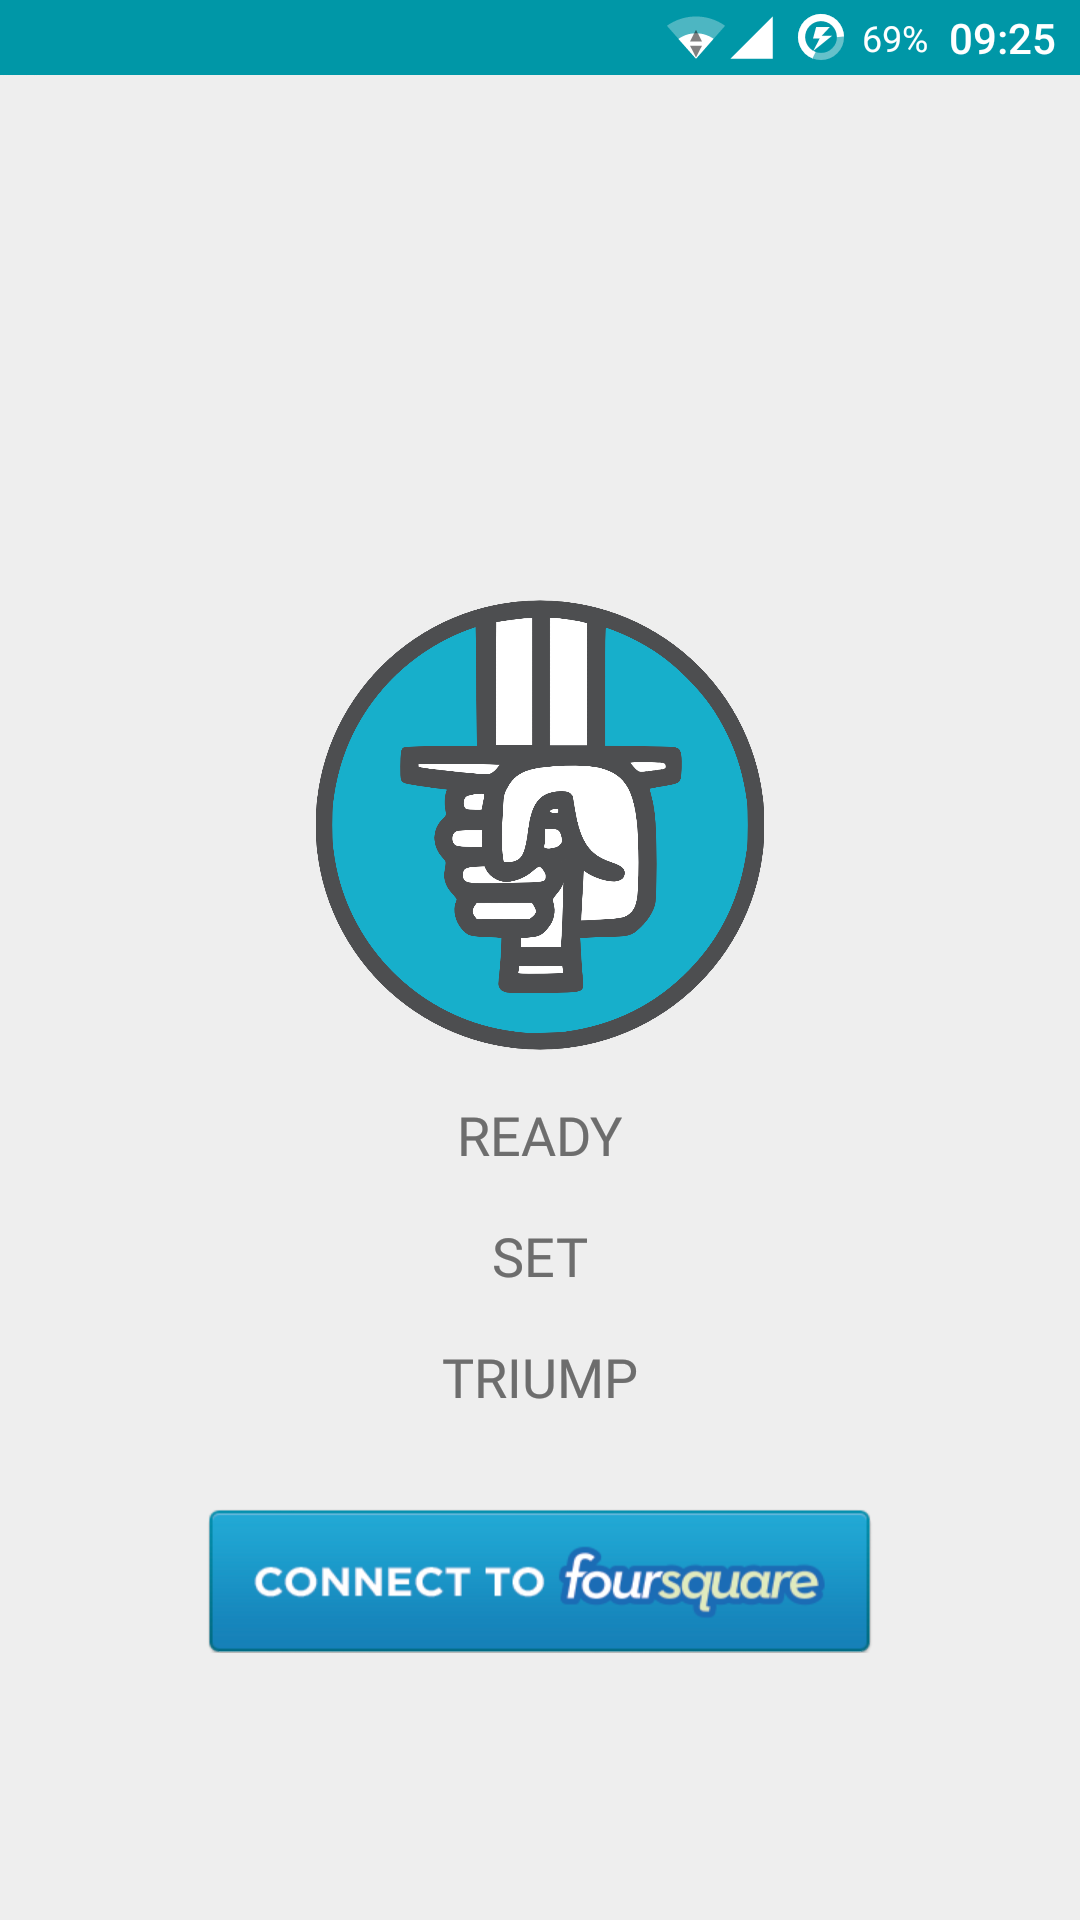
\includegraphics[width=\textwidth]{shot_login}
\caption{Login}
\label{fig:screenshot_profile}
\end{minipage}
\hspace{2.4cm}
\begin{minipage}[b]{0.20\linewidth}
\centering
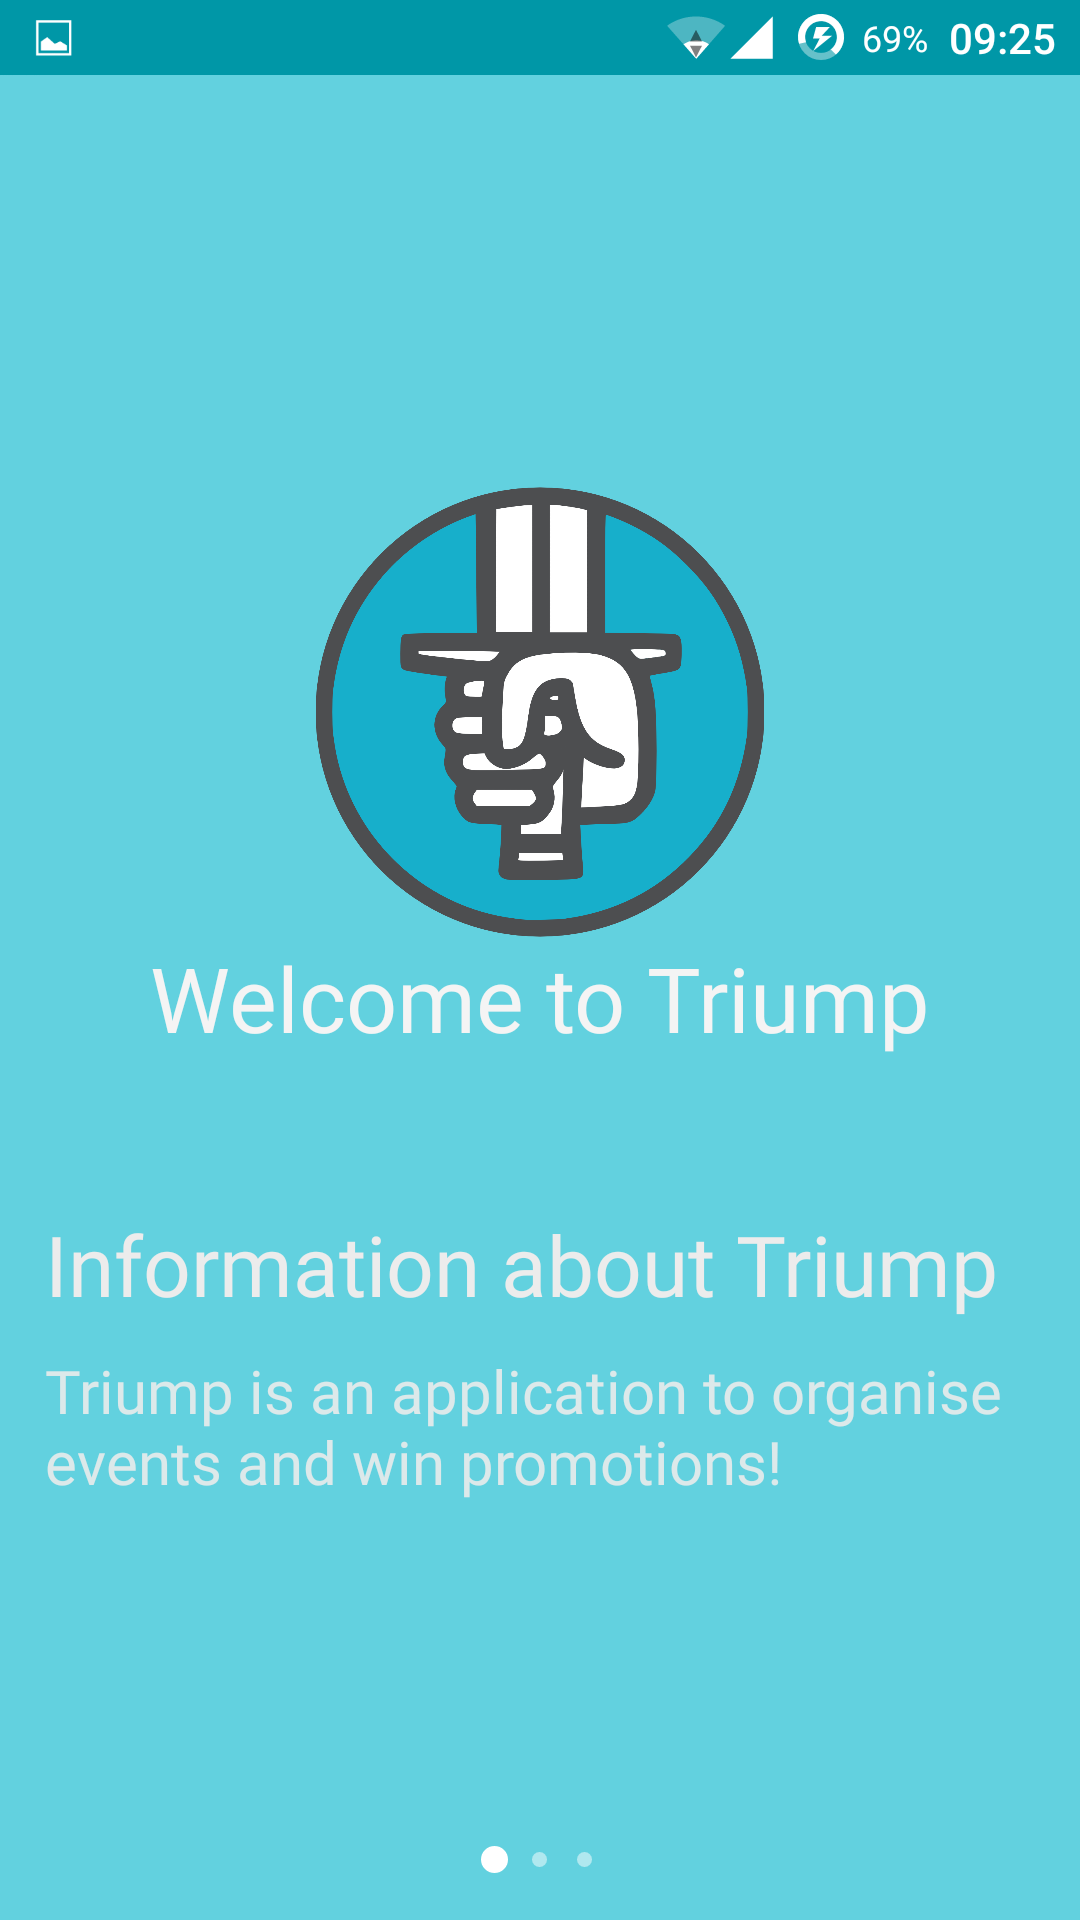
\includegraphics[width=\textwidth]{shot_tutorial}
\caption{Tutorial}
\label{fig:screenshot_login}
\end{minipage}
\hspace{2.4cm}
\begin{minipage}[b]{0.20\linewidth}
\centering
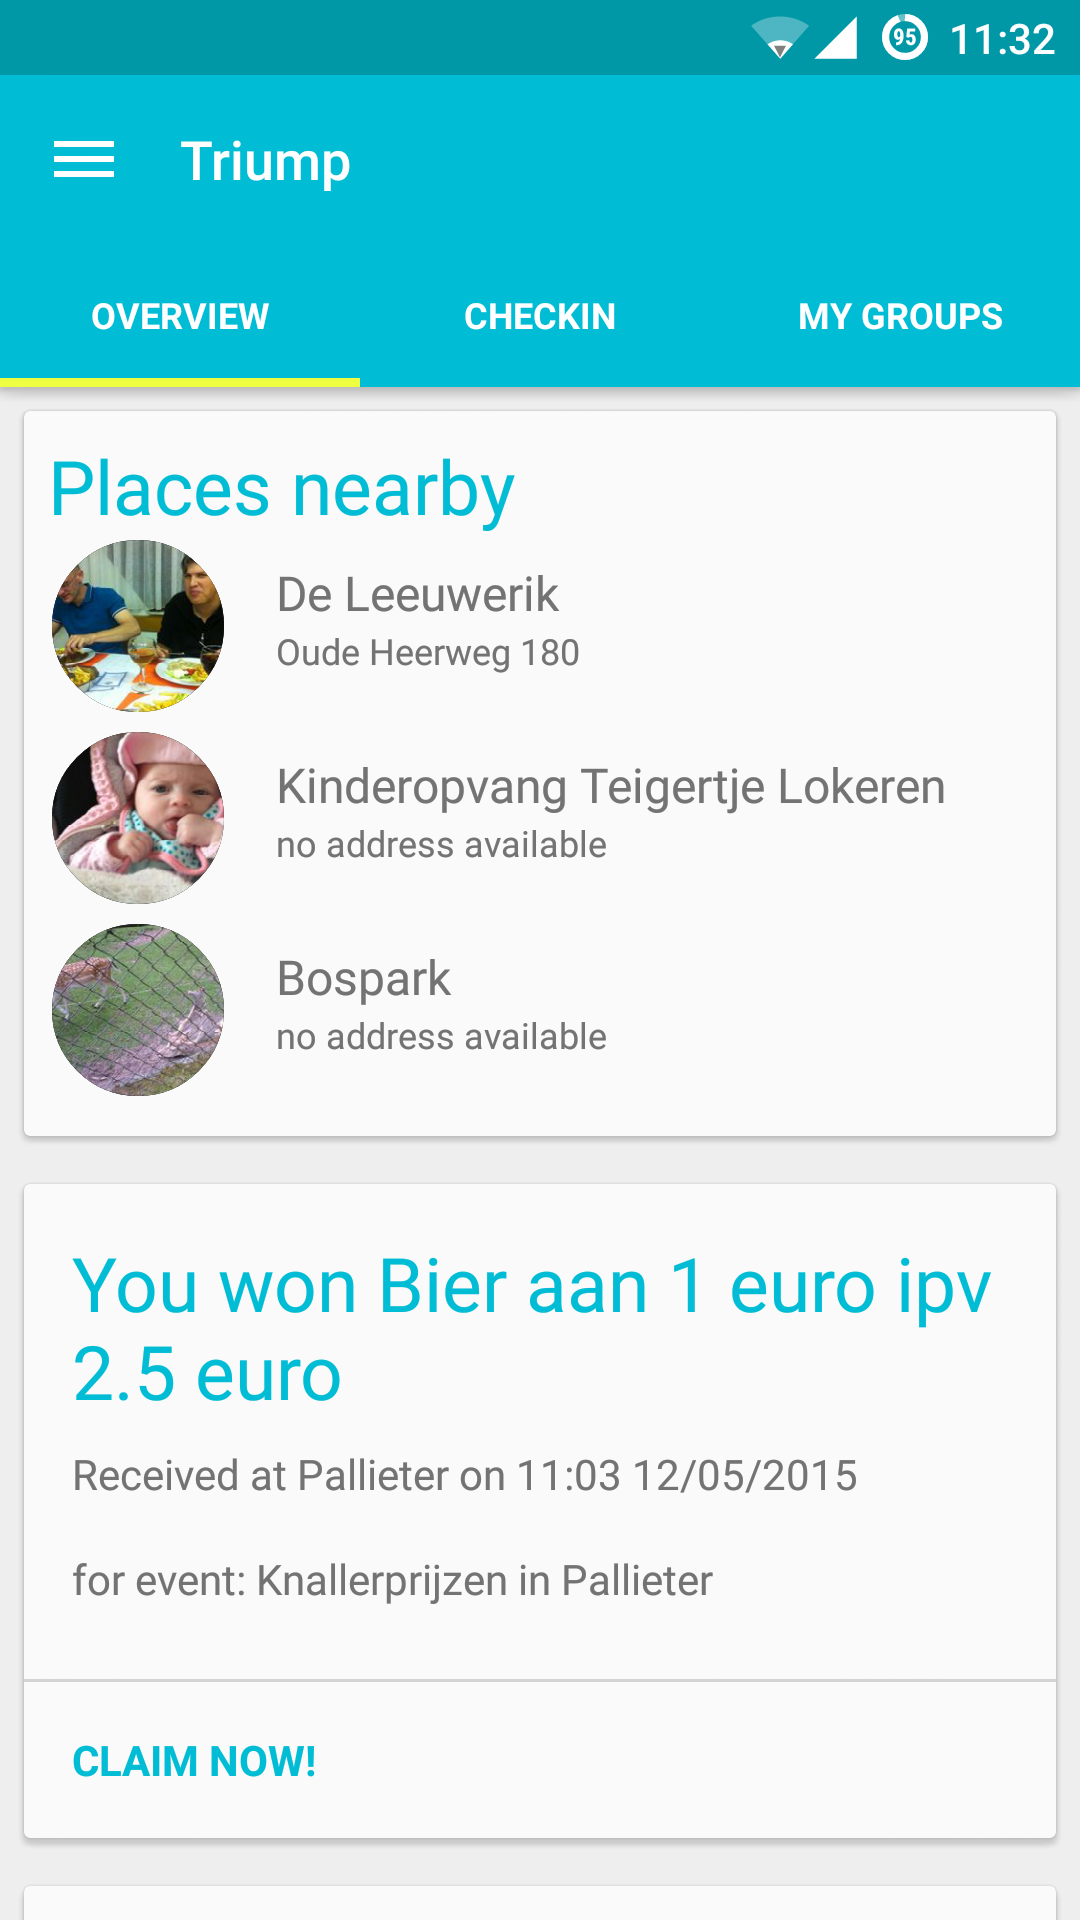
\includegraphics[width=\textwidth]{shot_overview1}
\caption{Overzicht}
\label{fig:screenshot_overview}
\end{minipage}
\end{figure}
\clearpage
\subsubsection{Overview en notificaties} %Lars
Om gebruikers op de hoogte te houden van recente activiteit van hun groepen, events die aan de gang zijn, promoties, checkins,... worden in de Android applicatie 2 mechanismen voorzien. 
Enerzijds is er het Overviewscherm, het eerste scherm dat de gebruiker ziet in de applicatie, anderzijds zijn er de notificaties.
Het Overviewscherm wordt dynamisch gegenereerd op basis van de activiteit van de gebruikers. Hiervoor wordt met `CardViews' in een RecyclerView gewerkt, waardoor ze efficiënt kunnen voorgesteld worden in een lijst en interactief zijn. Het Overviewscherm toont de checkins van groepsleden , evenementen in de buurt en gewonnen promoties. Op deze manier kan de gebruiker vanuit het Overviewscherm navigeren naar andere onderdelen binnen de applicatie (evenementen, ranglijsten, groepen, checkin...).
Naast het Overviewscherm, wordt de gebruiker van updates voorzien via notificaties. Deze notificaties hebben betrekking op evenementen en promoties (voor checkins worden geen notificaties verstuurd om de gebruiker niet te belasten met overbodige notificaties). Bovendien heeft de gebruiker de mogelijkheid om notificaties uit te schakelen via de instellingen. Notificaties kunnen ook occasioneel gebruikt worden om aan de gebruiker feedback te vragen via het Feedbackscherm. Voornamelijk in de ontwikkel- en testfase is dit van belang.
Kortom, het Overviewscherm en de notificaties zijn een interactieve manier om de gebruikers aan te zetten tot het gebruiken van de applicatie.

\subsubsection{Checkin}%Siebe
Om integratie met de diensten van Swarm te voorzien wordt een gelijkaardige interface om in te checken gebruikt. Een Location service controleert de locatie van de gebruiker en toont op de kaart de naburige Foursquare locaties. De gebruiker kan vervolgens uit een dynamisch schaalbare lijst de locatie kiezen waar men wil inchecken. Indien de gebruiker niet geïnteresseerd is om in te inchecken, maar enkel de ranglijsten of evenementen wil controleren op een bepaalde locatie, kan dit door de locatie in te typen in het zoekveld. Bij het selecteren van een locatie (via de kaart of via de zoekfunctionaliteit) krijgt de gebruiker een overzicht van de locatie. Dit overzicht bestaat steeds uit 2 onderdelen, namelijk de ranglijsten en de evenementen. De gebruiker kan van ranglijst wisselen (voor verschillende groottes of types van groepen). Daarnaast kan de gebruiker, indien hij voldoende dicht is bij de locatie , inchecken voor zijn groepen. Indien de gebruiker een locatie via de zoekfunctionaliteit heeft opgezocht, maar te zich hiervan te ver bevindt, is inchecken niet mogelijk. Men kan wel steeds  de verschillende evenementen te bekijken in het Event onderdeel.
\begin{figure}[ht]
\begin{minipage}[b]{0.25\linewidth}
\centering
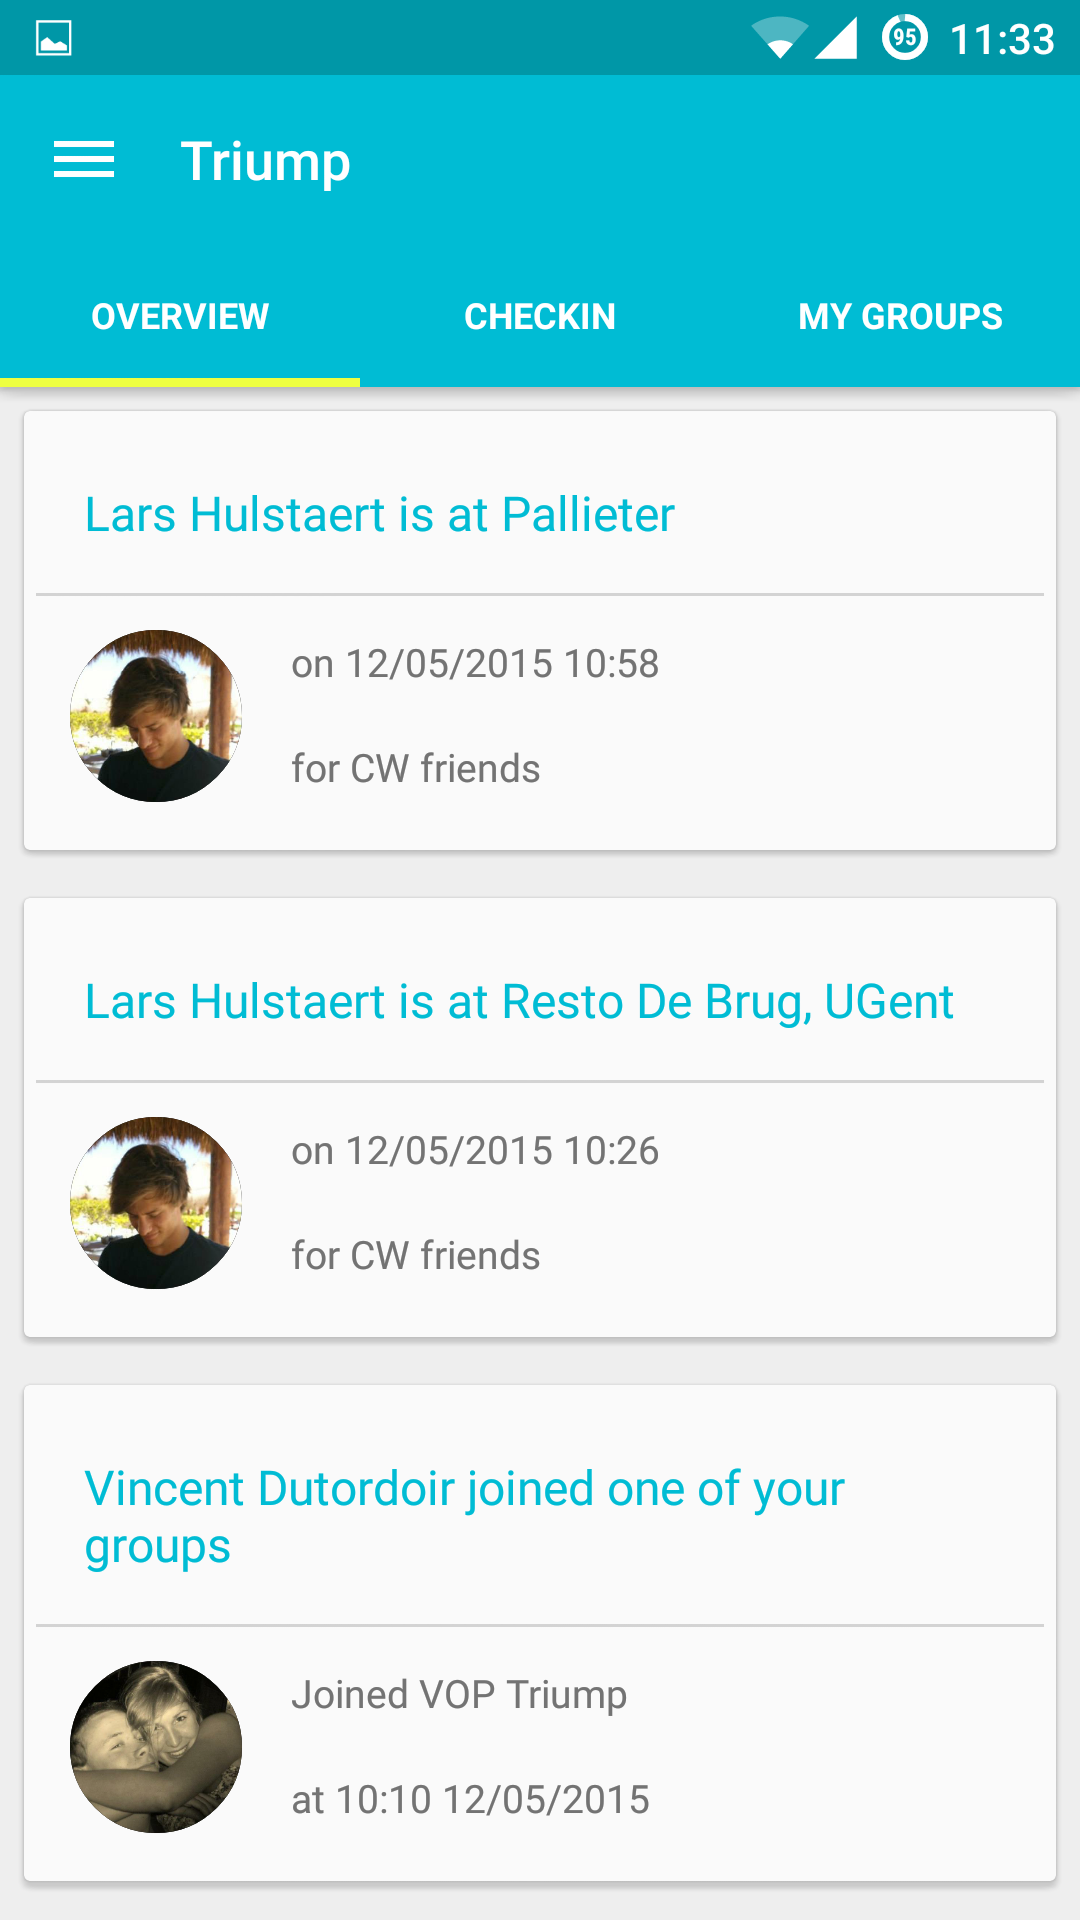
\includegraphics[width=\textwidth]{shot_overview2}
\caption{Overzicht}
\label{fig:screenshot_overview2}
\end{minipage}
\hspace{1.5cm}
\begin{minipage}[b]{0.25\linewidth}
\centering
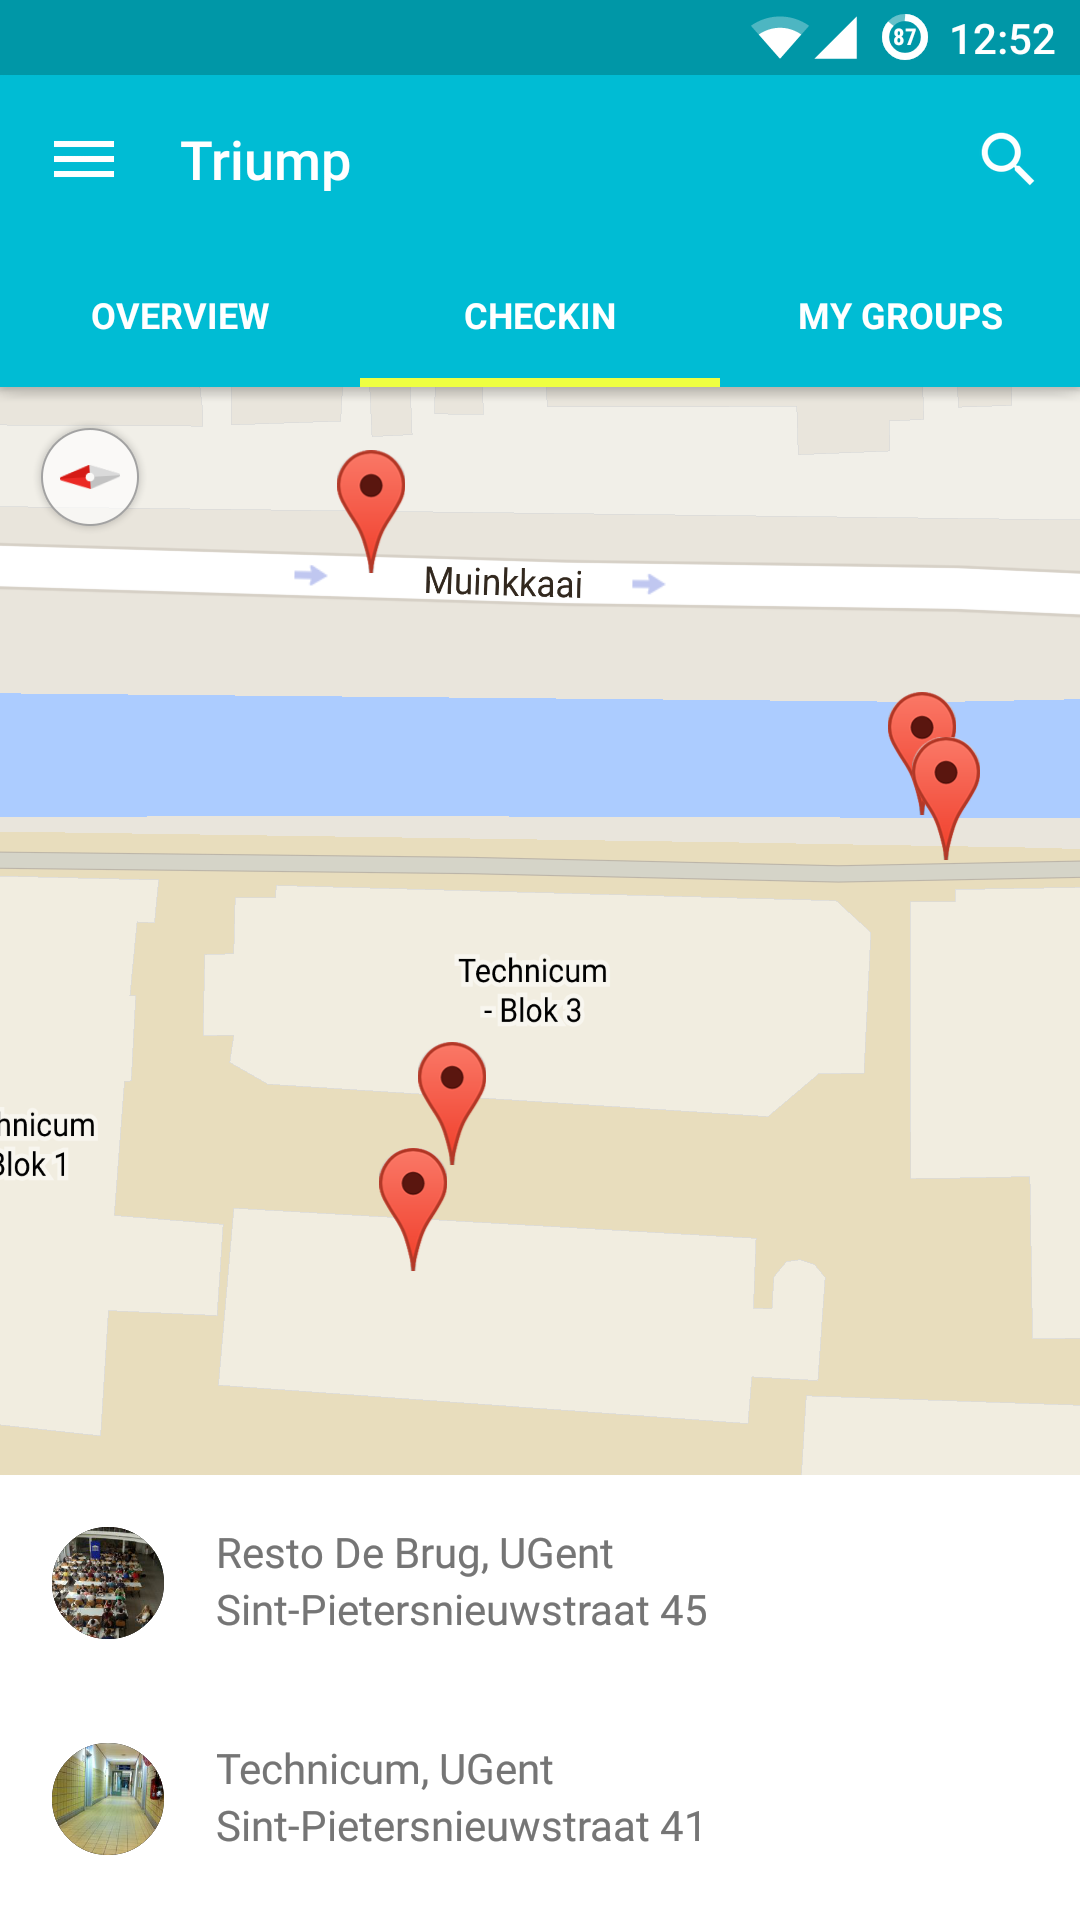
\includegraphics[width=\textwidth]{shot_checkin}
\caption{Checkin}
\label{fig:screenshot_checkin}
\end{minipage}
\hspace{1.5cm}
\begin{minipage}[b]{0.25\linewidth}
\centering
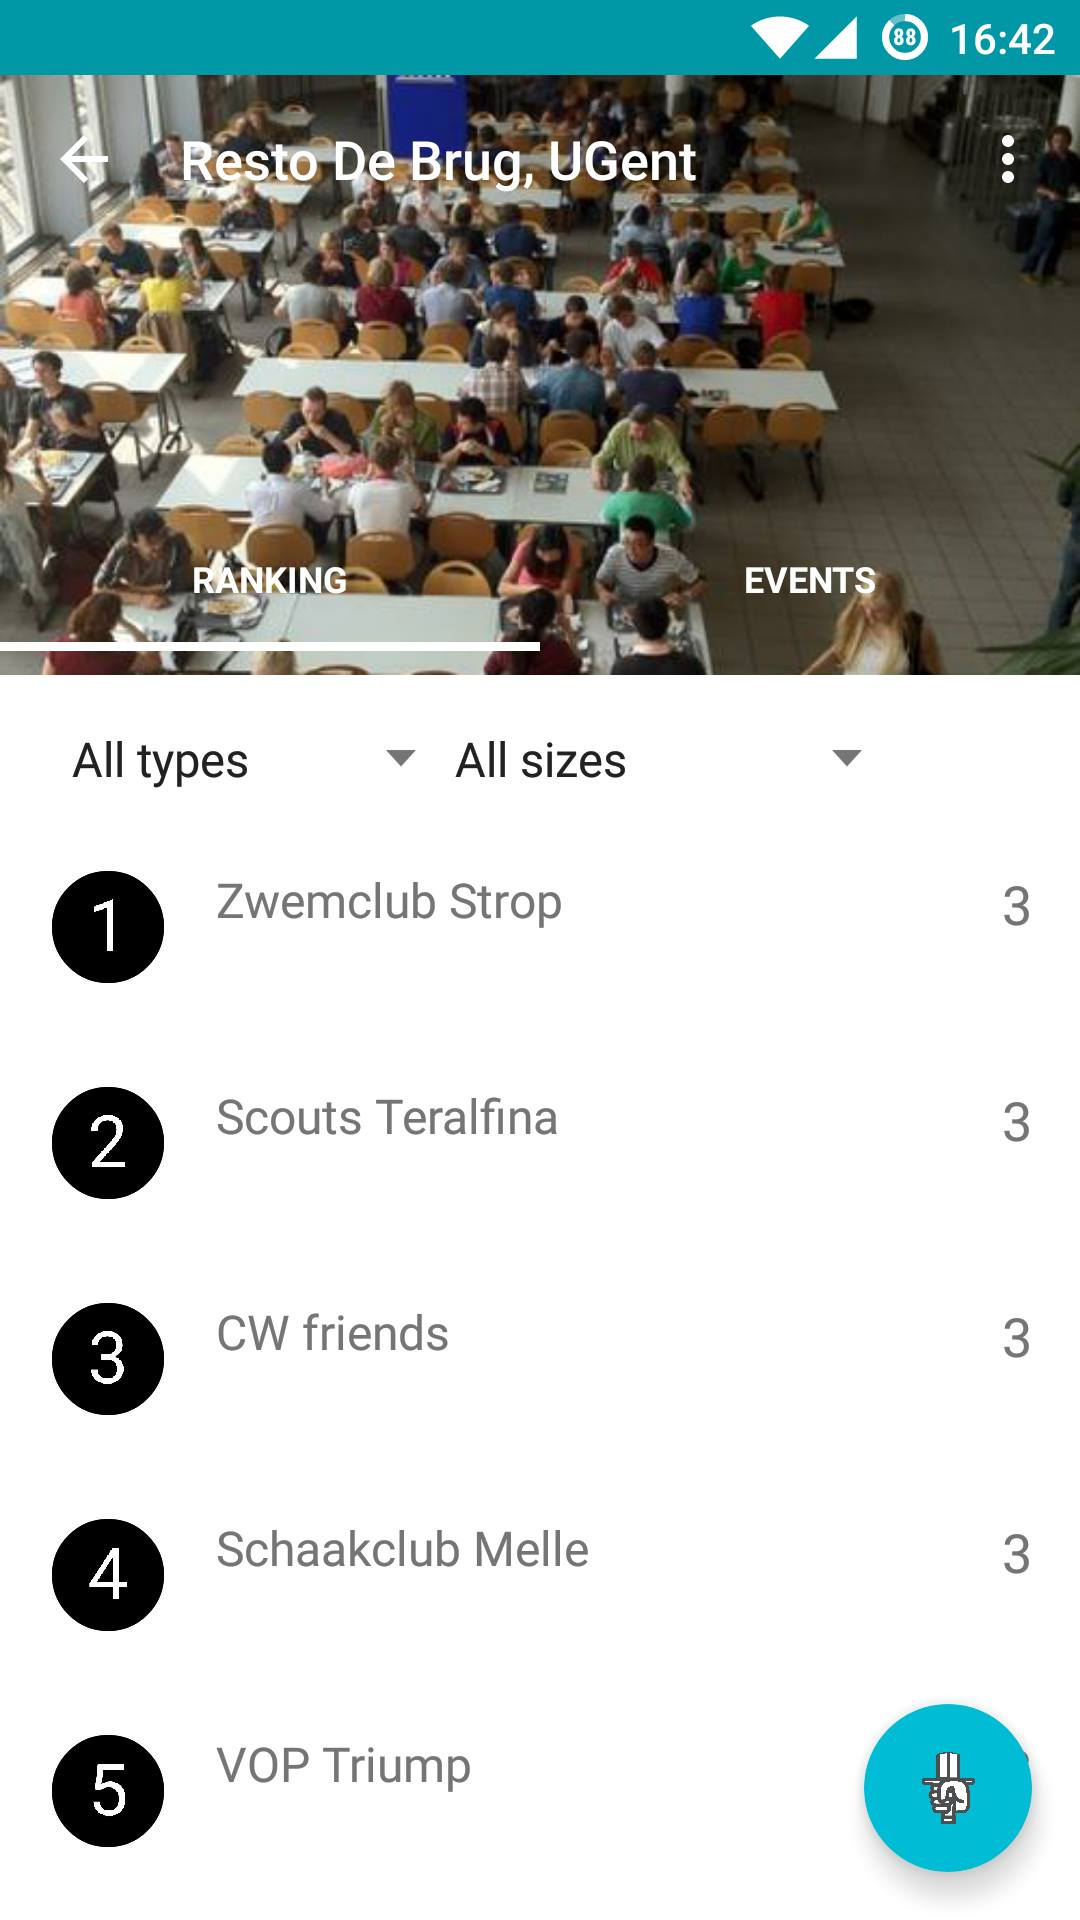
\includegraphics[width=\textwidth]{shot_venue}
\caption{Locatie}
\label{fig:screenshot_venue}
\end{minipage}
\end{figure}
\clearpage
\subsubsection{Groepen}%Lars
Een belangrijk onderdeel van de Triump applicatie is het groepsaspect. Groepen kunnen vanuit de toepassing zelf aangemaakt worden, en opgezocht worden. Daarnaast kunnen leden zich inschrijven voor groepen, en adminstrators kunnen deze aanvaarden. Vanop de startpagina kan de gebruiker de activiteit van groepsleden bekijken en navigeren naar zijn eigen groepen. Ranglijsten en evenementen steunen steeds op dit groepsprincipe in de zin dat de entiteiten waarvoor ranglijsten en evenementen opgesteld worden steeds groepen zijn. Dezelfde functionaliteit is ook mogelijk vanuit de webinterface (in het geval dat gebruik op de smartphone te onoverzichtelijk wordt).

\begin{figure}[ht]

\begin{minipage}[b]{0.25\linewidth}
\centering
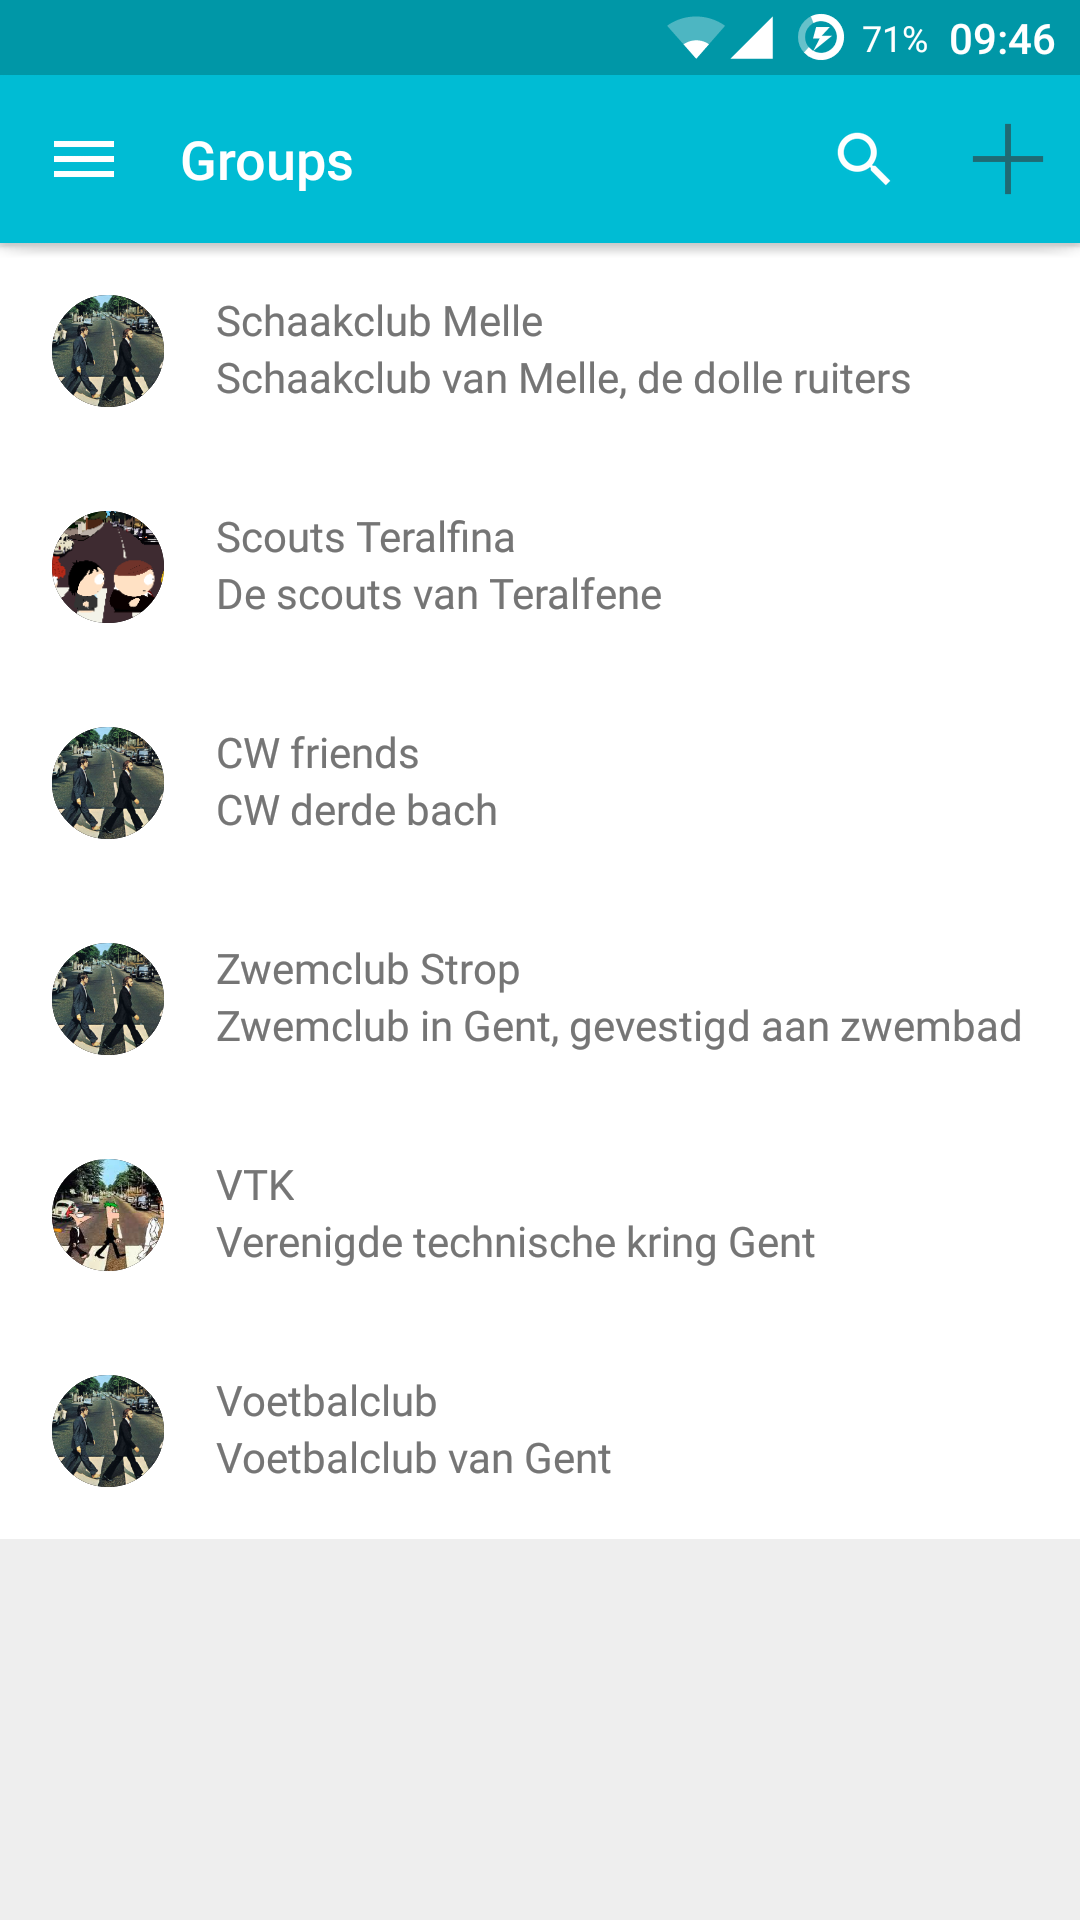
\includegraphics[width=\textwidth]{shot_groups}
\caption{Groepen bekijken}
\label{fig:shot_groups}
\end{minipage}
\hspace{1cm}
\begin{minipage}[b]{0.25\linewidth}
\centering
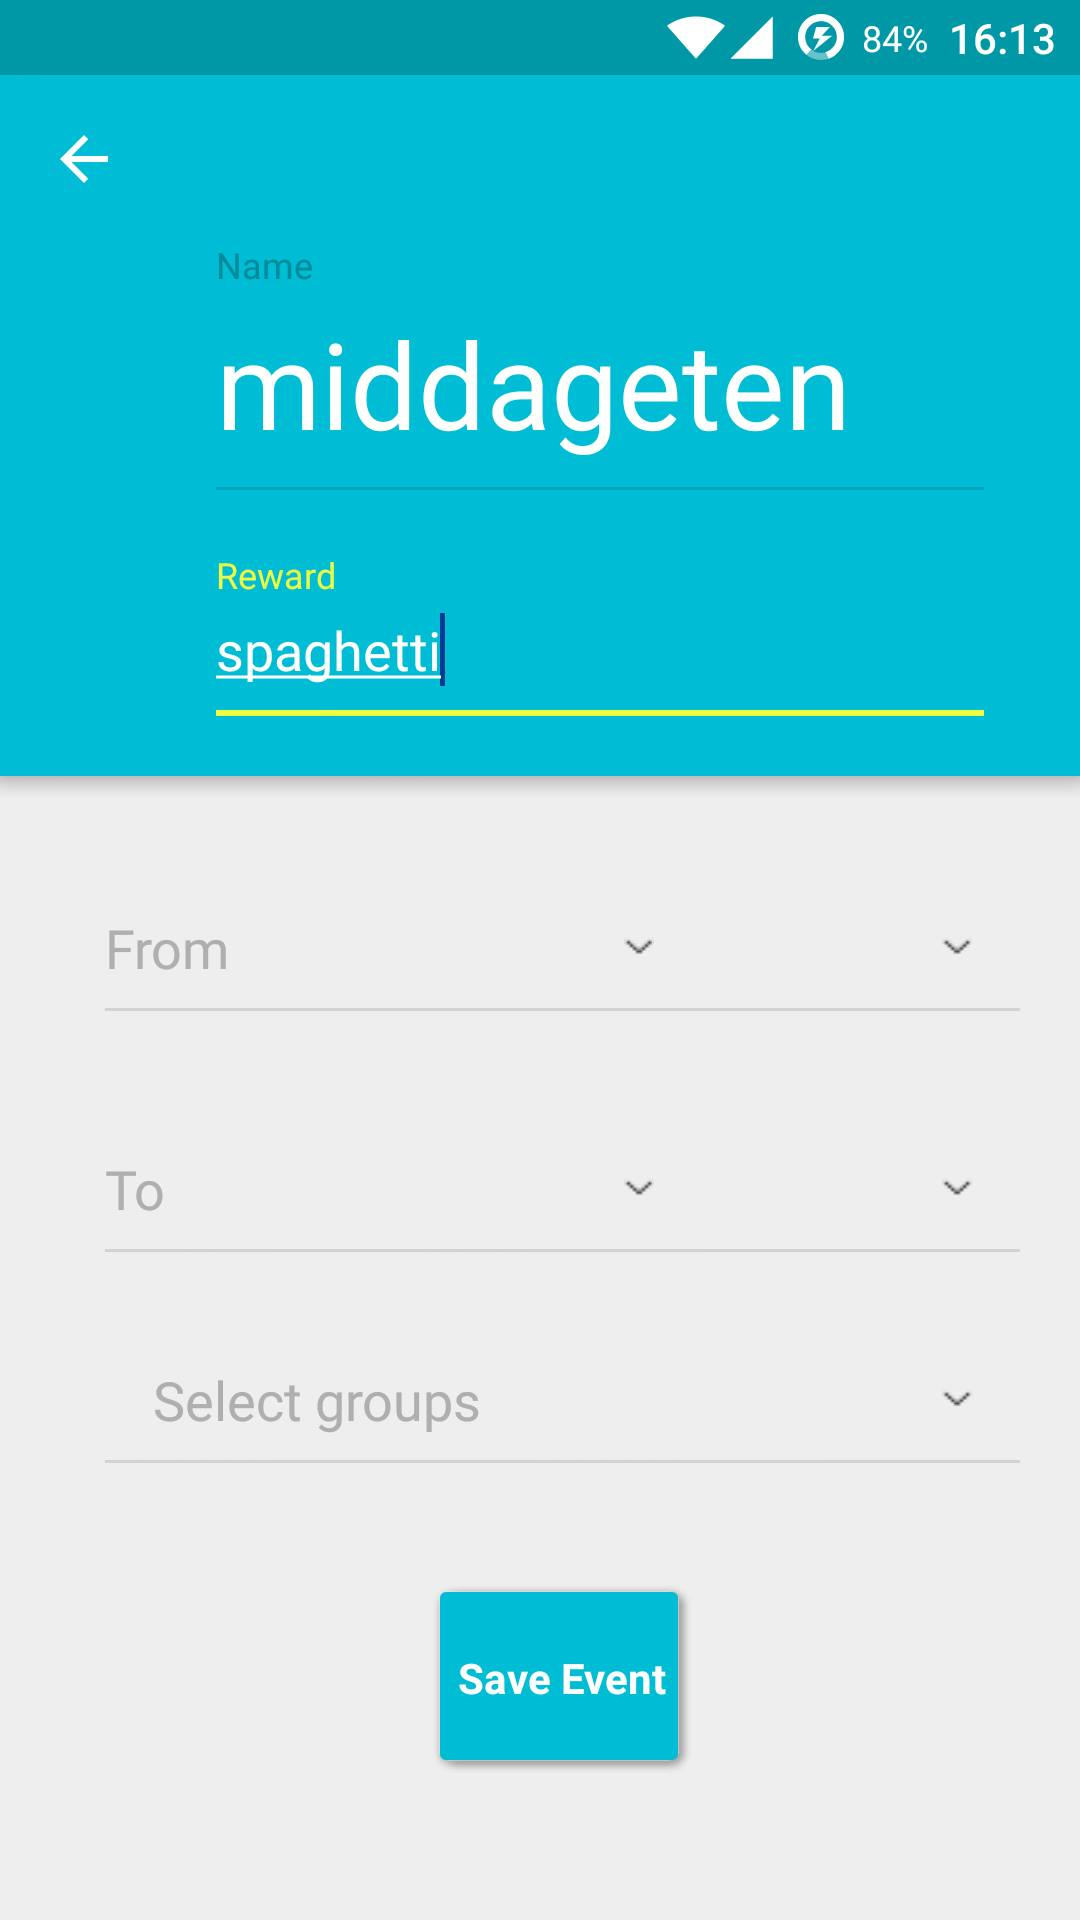
\includegraphics[width=\textwidth]{shot_groep_aanmaken}
\caption{Groep aanmaken}
\label{fig:shot_groep_aanmaken}
\end{minipage}
\hspace{1cm}
\begin{minipage}[b]{0.25\linewidth}
\centering
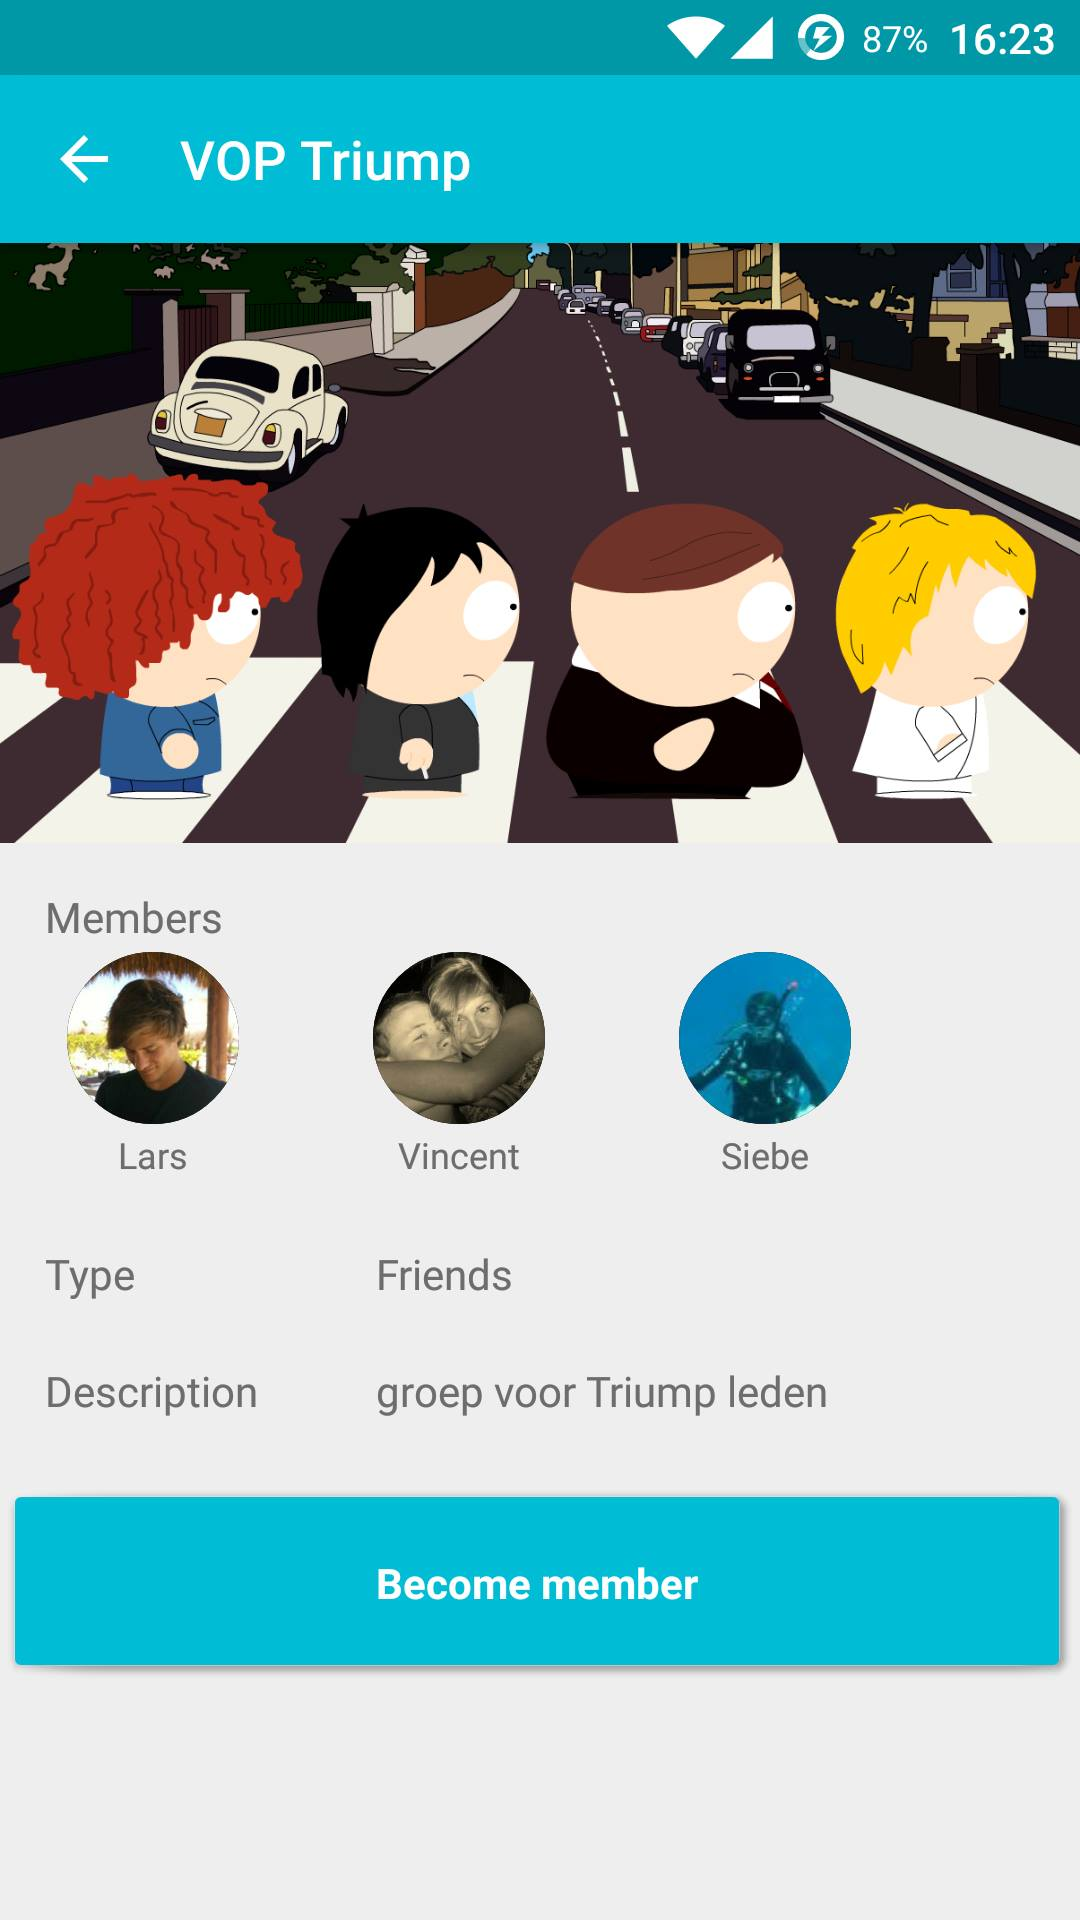
\includegraphics[width=\textwidth]{shot_group}
\caption{Groep-informatie}
\label{fig:shot_group}
\end{minipage}

\end{figure}

% % % % % % % % % % % % % % % % % % % % %
% afbeeldingen 2
\begin{figure}[ht]
\centering
\begin{minipage}[b]{0.5\linewidth}
\centering
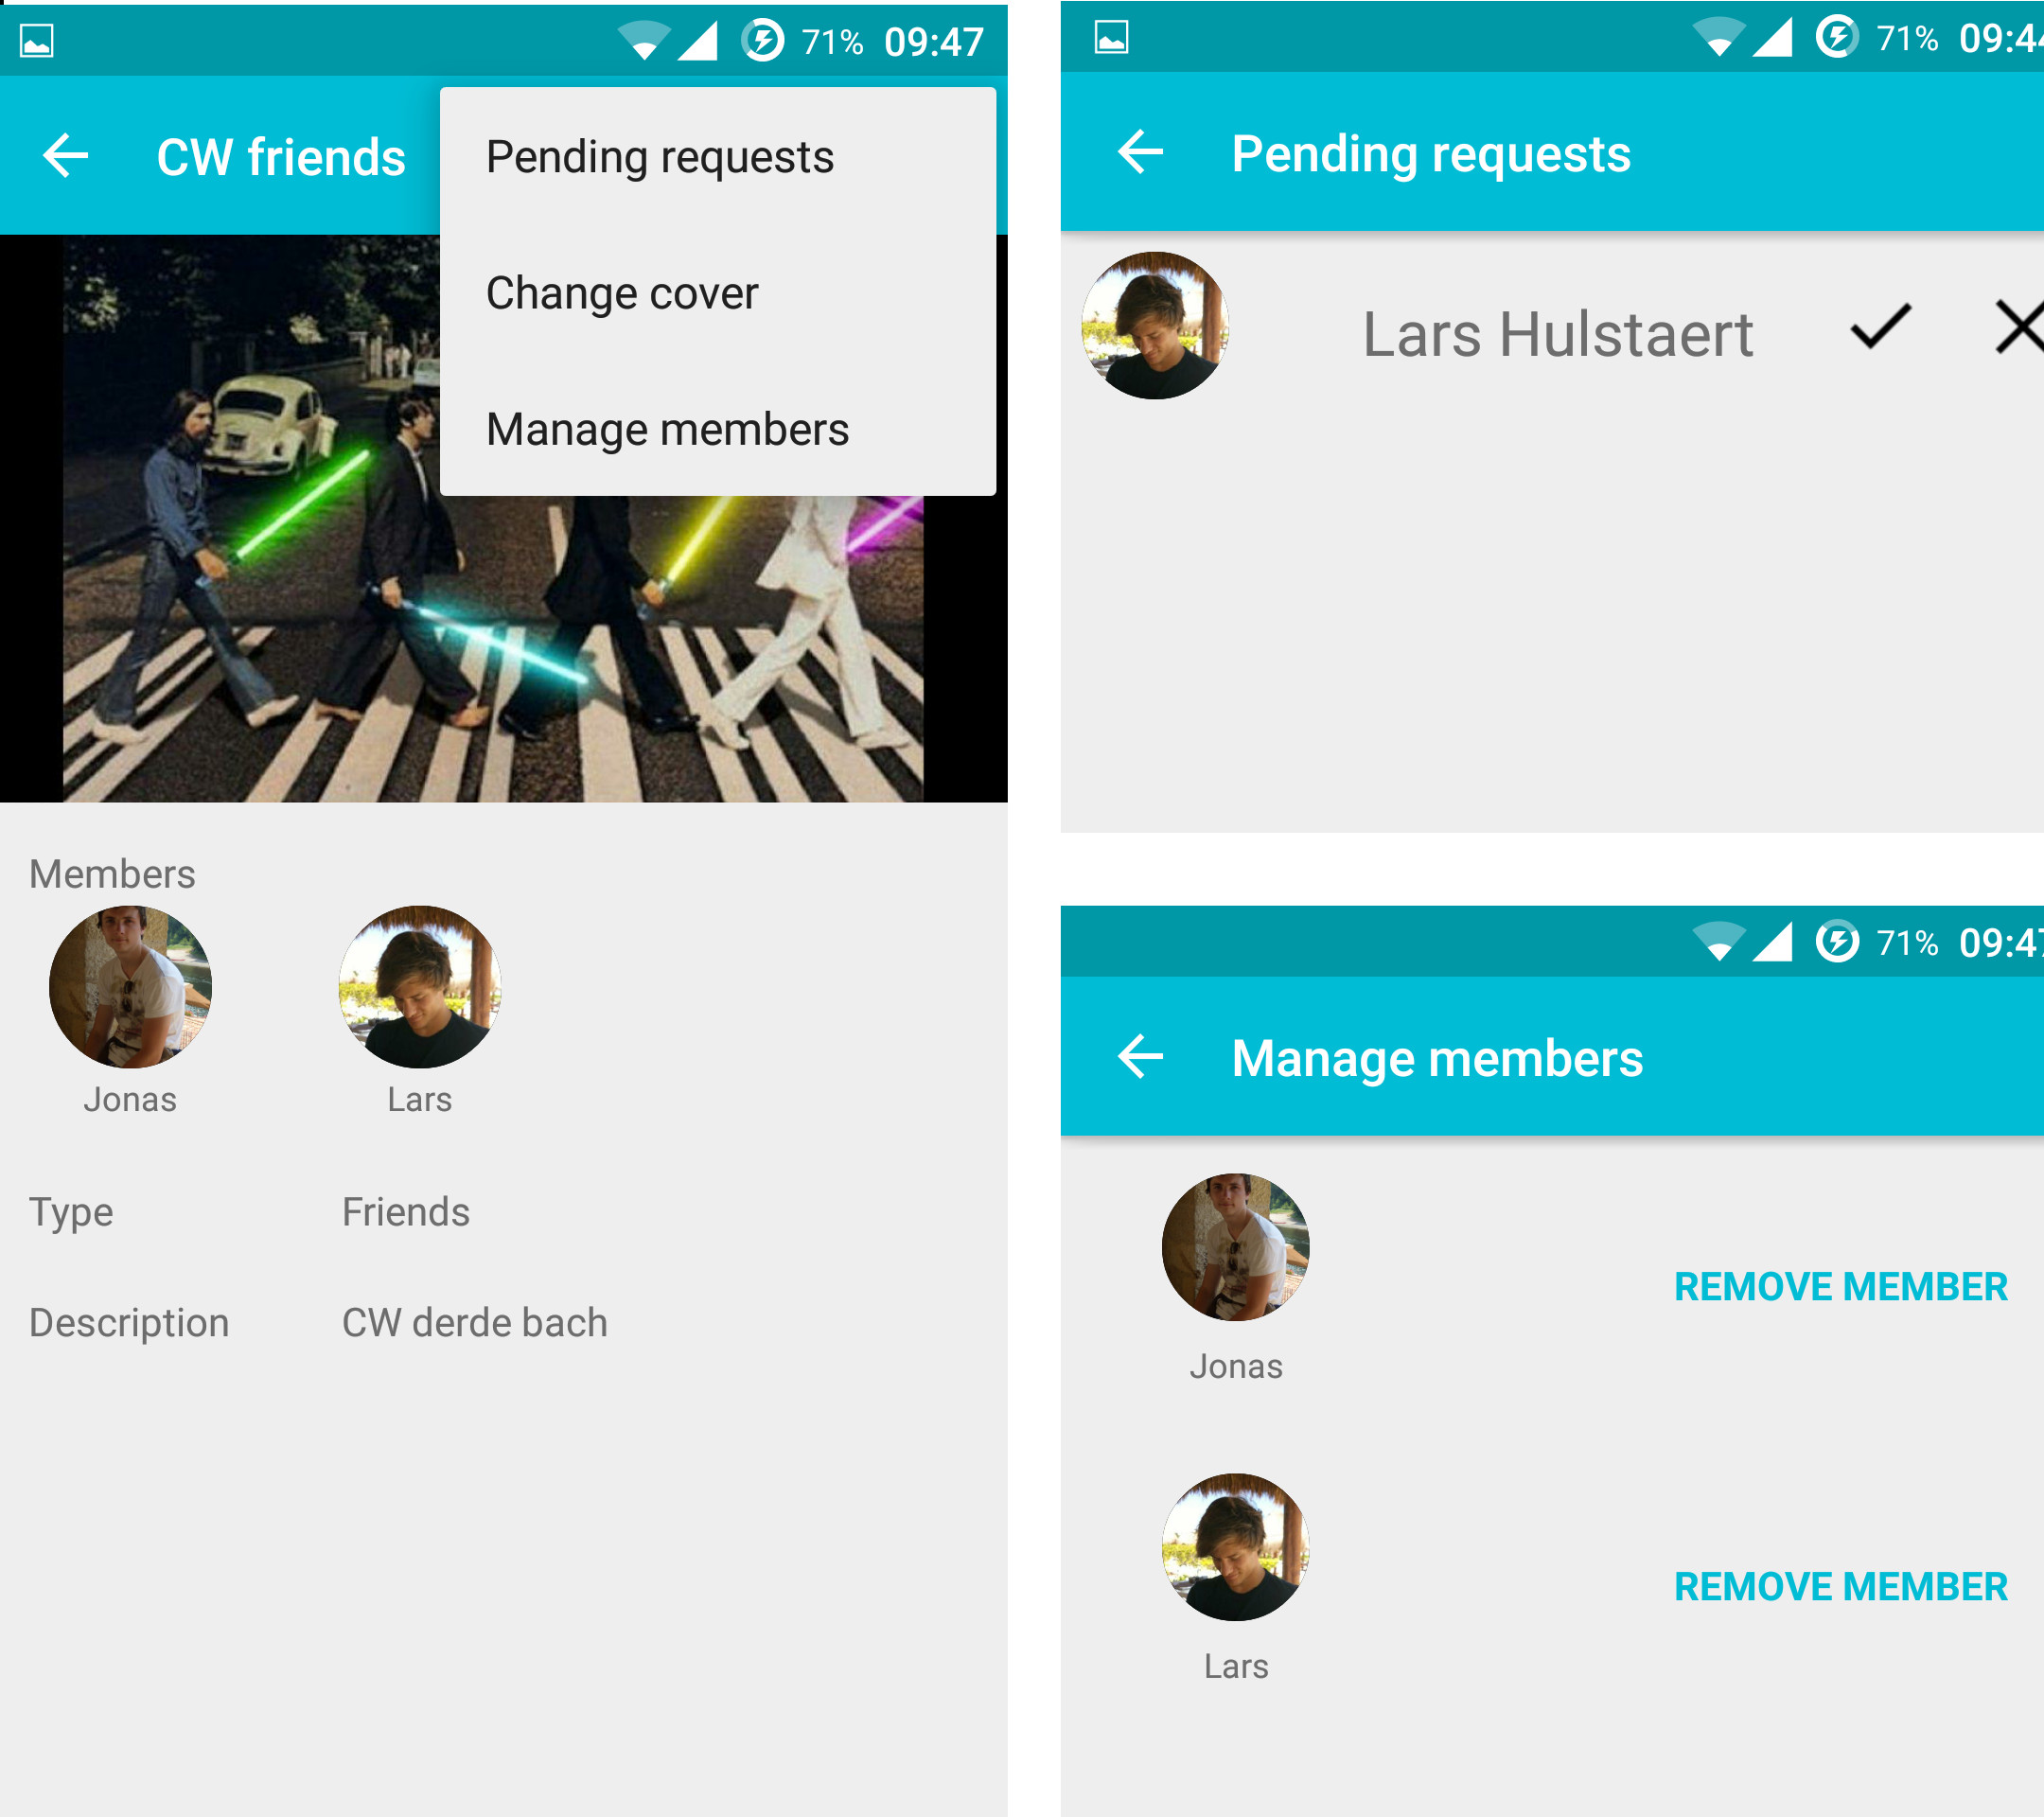
\includegraphics[width=\textwidth]{shot_groep_beheer}
\caption{Beheer groep. Accepteer lidschapverzoeken en verwijder leden}
\label{fig:shot_groep_beheer}
\end{minipage}


\end{figure}

\clearpage

\subsubsection{Events en Rewards}%Siebe
In het Eventsscherm krijgt de gebruiker een overzicht van alle evenementen. Hierbij worden officiële en niet-officiële in dezelfde lijst weergegeven maar worden ze grafisch onderscheiden. Het Eventsscherm is geïmplementeerd om te vermijden dat gebruikers via de locaties op zoek moet gaan naar evenementen.
In het Rewardscherm kan de gebruiker de promoties van officiële evenementen gaan opeisen indien hij/zij deze heeft gewonnen met één van zijn groepen. Momenteel kan de gebruiker beloningen opeisen door over een promotie te vegen, waarbij een dialoogscherm wordt geopend. Door dit scherm aan de eigenaar te tonen, kan vervolgens de beloning geïnd worden. Als uitbreiding kan er eventueel voor gezorgd worden dat de eigenaar een unieke afbeelding uploadt per promotie. Door te vegen over de promotie kan de afbeelding dan bv. 10 s getoond worden.
\subsubsection{Leaderboard}%Lars
Het Leaderboardscherm toont een algemene ranglijst. Deze ranglijst is onafhankelijk van een locatie en toont welke groepen zich globaal aan de leiding bevinden op basis van het aantal checkins. Momenteel wordt deze ranglijst nog in hetzelfde formaat getoond als bij de locaties. Een mogelijke uitbreiding is echter om naast een lijst te tonen, ook een kaartje te tonen dat dynamisch gegenereerd. Deze kaart zou dan per locatie tonen welke groep hier aan de leiding staat.De leaderboards kunnen gewijzigd worden afhankelijk van grootte en type van de groepen.



\subsubsection{Notificaties} %Vincent
Het notificatiesysteem zorgt ervoor dat gebruikers verwittigd worden van belangrijke gebeurtenissen binnen Triump en met slechts één beweging de betreffende pagina kunnen waarnemen. In de huidige implementatie zal een gebruiker een notificatie ontvangen indien een groep waartoe hij/zij behoort een evenement heeft gewonnen. Wanneer er op de notificatie wordt geklikt zal de evenementpagina meteen worden getoond. Daarnaast kan een gebruiker ook via notificaties aangespoord worden om feedback te verschaffen.   

\begin{figure}[ht]

\begin{minipage}[b]{0.25\linewidth}
\centering
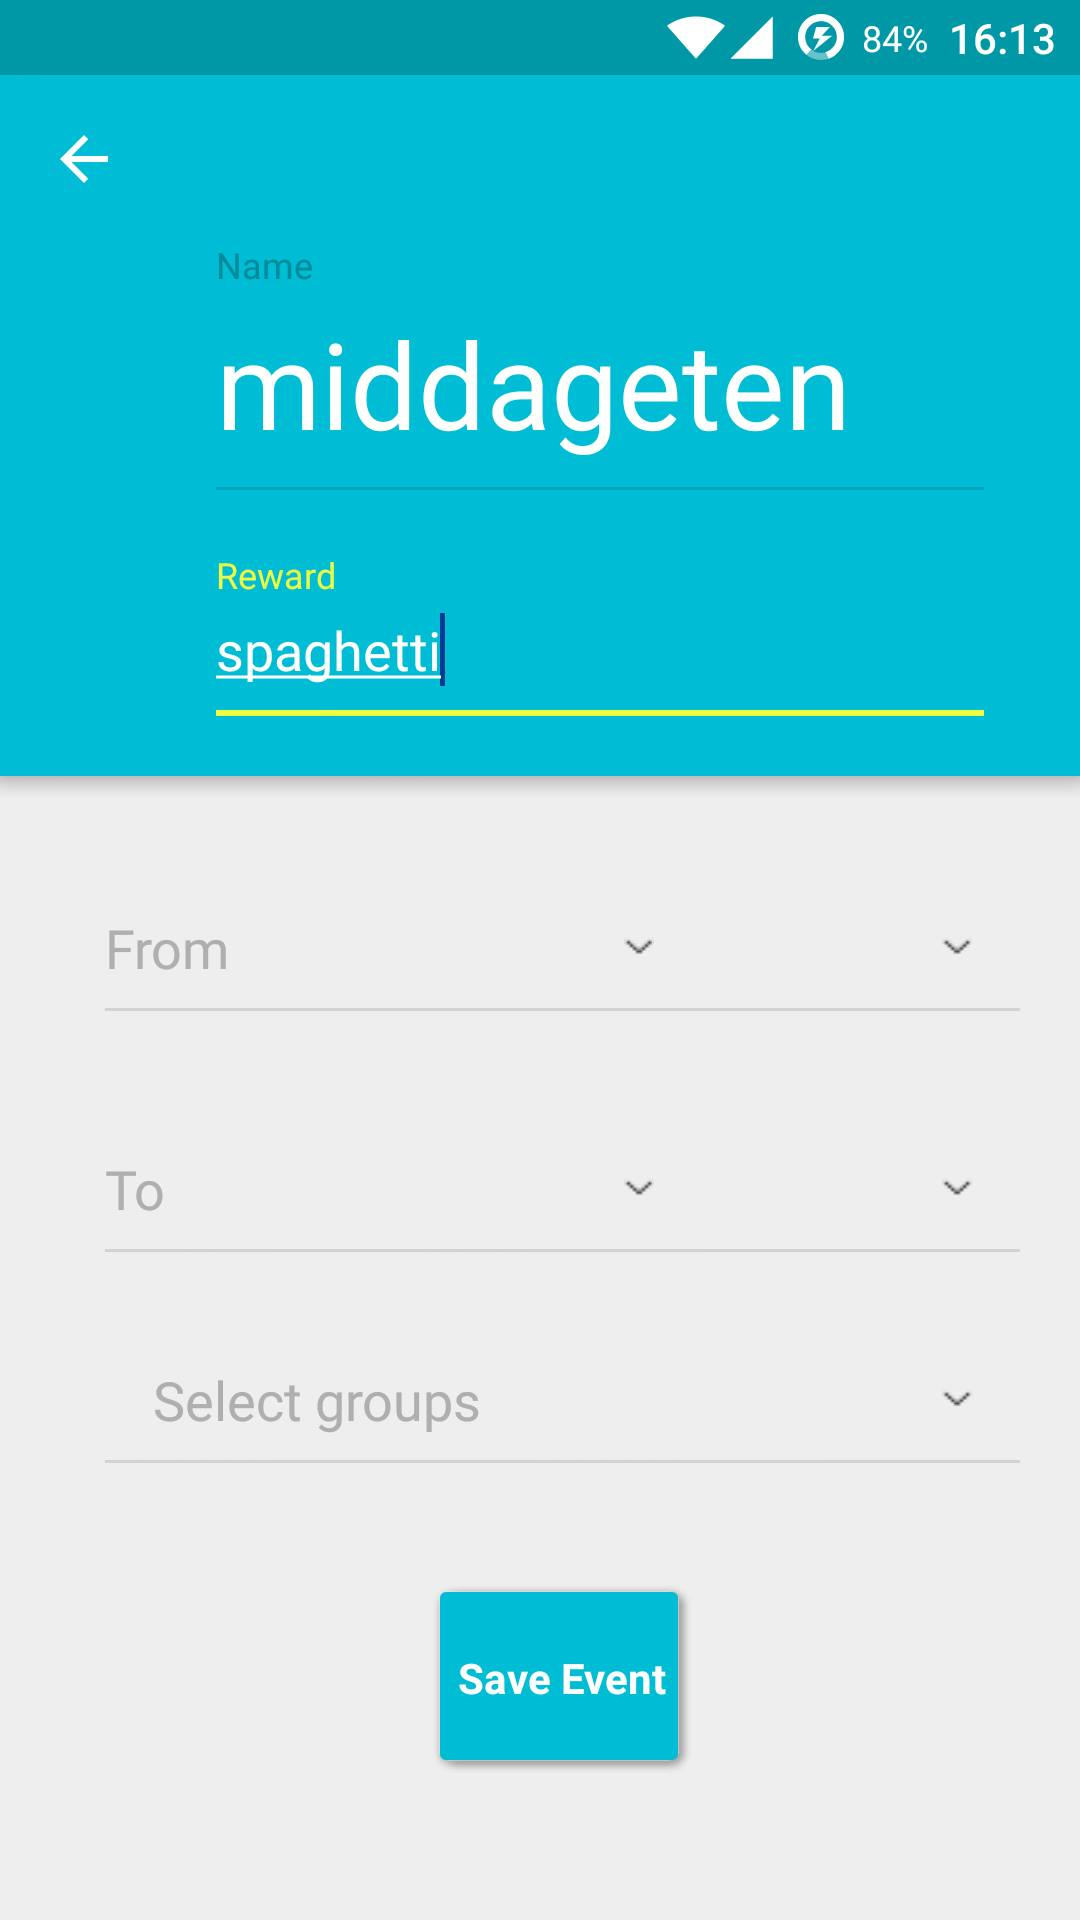
\includegraphics[width=\textwidth]{shot_event_aanmaken}
\caption{Event aanmaken}
\label{fig:shot_event_aanmaken}
\end{minipage}
\hspace{1.8cm}
\begin{minipage}[b]{0.25\linewidth}
\centering
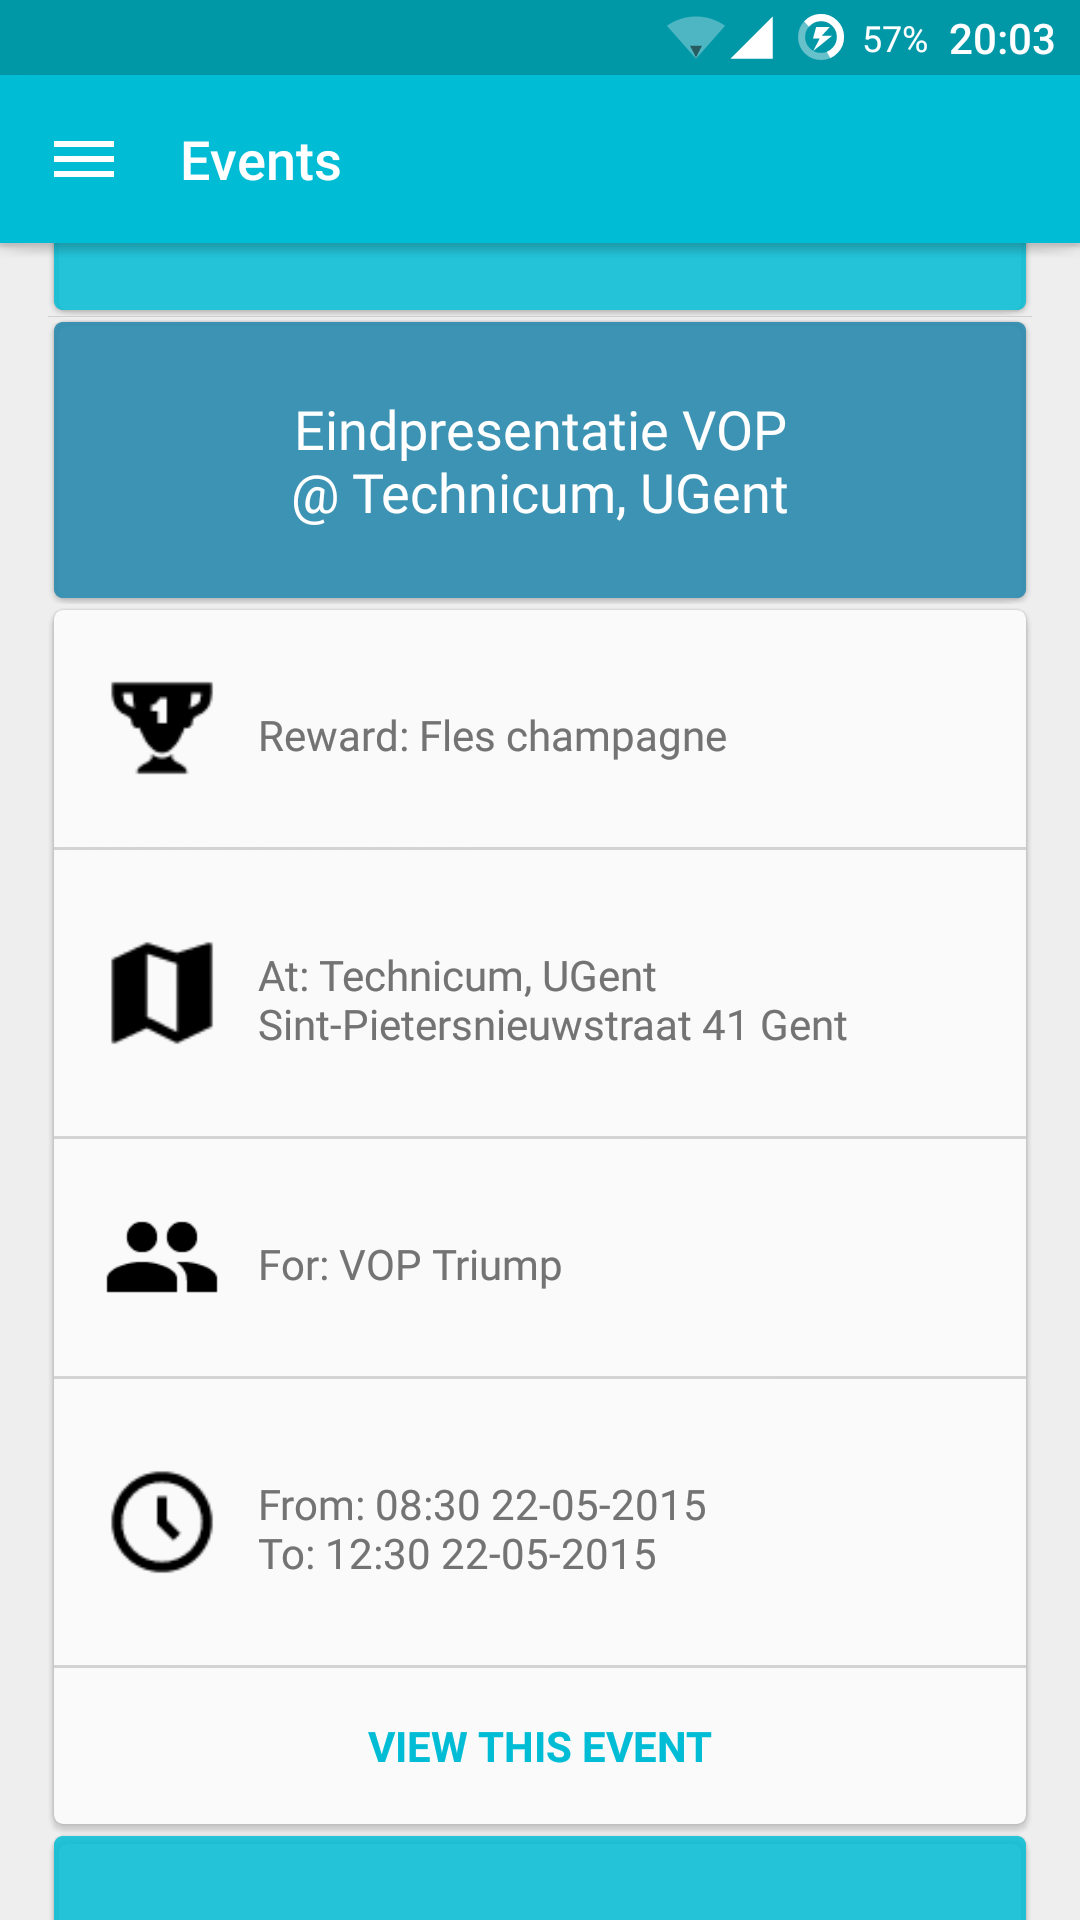
\includegraphics[width=\textwidth]{shot_event}
\caption{Event-informatie}
\label{fig:shot_event}
\end{minipage}
\hspace{1.8cm}
\begin{minipage}[b]{0.25\linewidth}
\centering
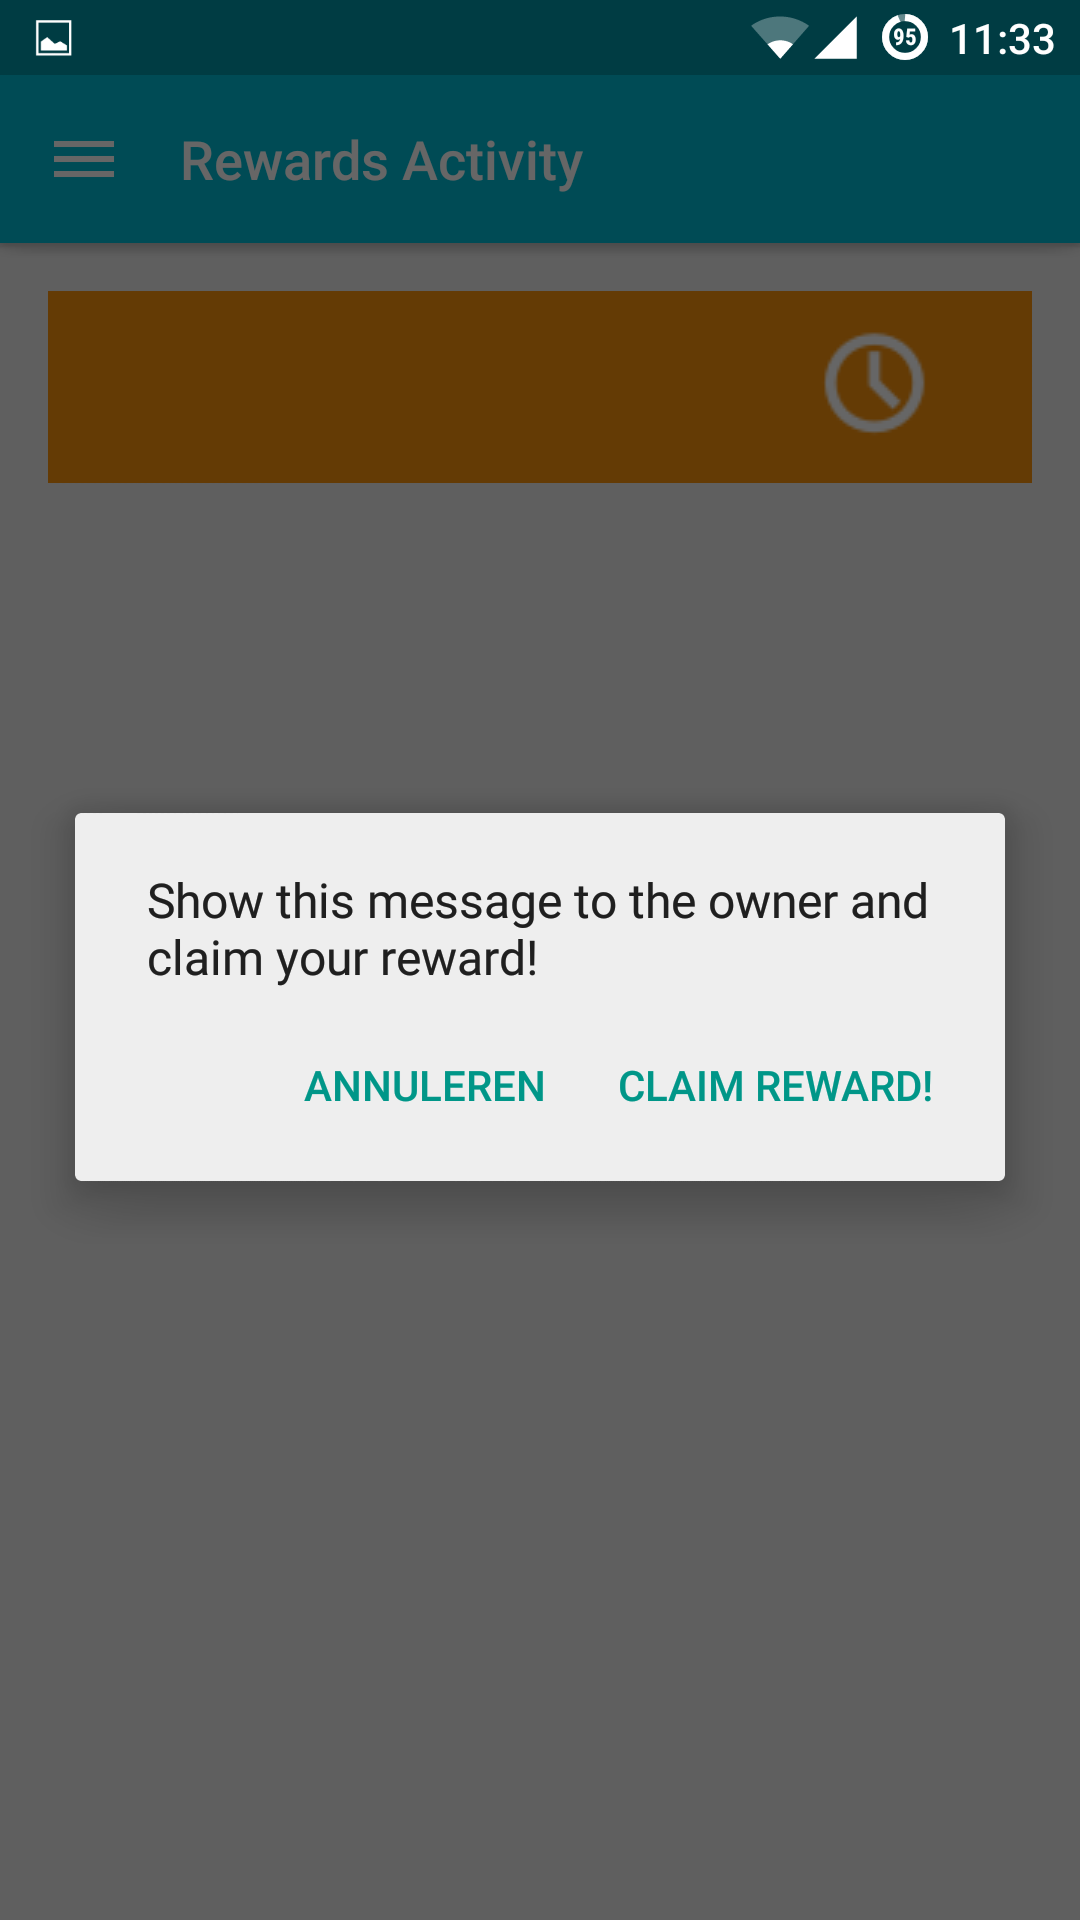
\includegraphics[width=\textwidth]{shot_reward_claim}
\caption{Ontvang promotie}
\label{fig:shot_reward_claim}
\end{minipage}
\end{figure}
\clearpage

\subsubsection{Feedback}%Siebe
In de ontwikkelfase, maar ook bij het uitbrengen van een eerste versie van de toepassing is feedback van cruciaal belang. Om het testgebruikers mogelijk te maken vanuit de applicatie zelf feedback te laten geven wordt een Feedbackscherm voorzien. De gebruiker kan in een tekstveld schrijven wat hij van Triump vindt en eventuele bugs melden. Deze berichten worden dan onmiddelijk doorgestuurd naar het gemeenschappelijk emailadres van Triump.
\subsubsection{Settings en profile}% Lars
Om de applicatie configureerbaar te maken wordt een instellingscherm voorzien. Hiervoor wordt de methode voorzien voorgeschreven door Google Applications.
Voorbeelden van instellingen in Triump zijn: het aan- en uitzetten van notificaties, het al dan niet delen van je profiel, het kleurenschema dat de applicatie gebruikt,...
% http://developer.android.com/guide/topics/ui/settings.html 
en deze hebben we dan ook gevolgd. Voorbeelden van instellingen in Triump zijn: het aan- en uitzetten van notificaties, het al dan niet delen van je profiel, het kleurenschema dat de applicatie gebruikt,...

\begin{figure}[ht]

\begin{minipage}[b]{0.25\linewidth}
\centering
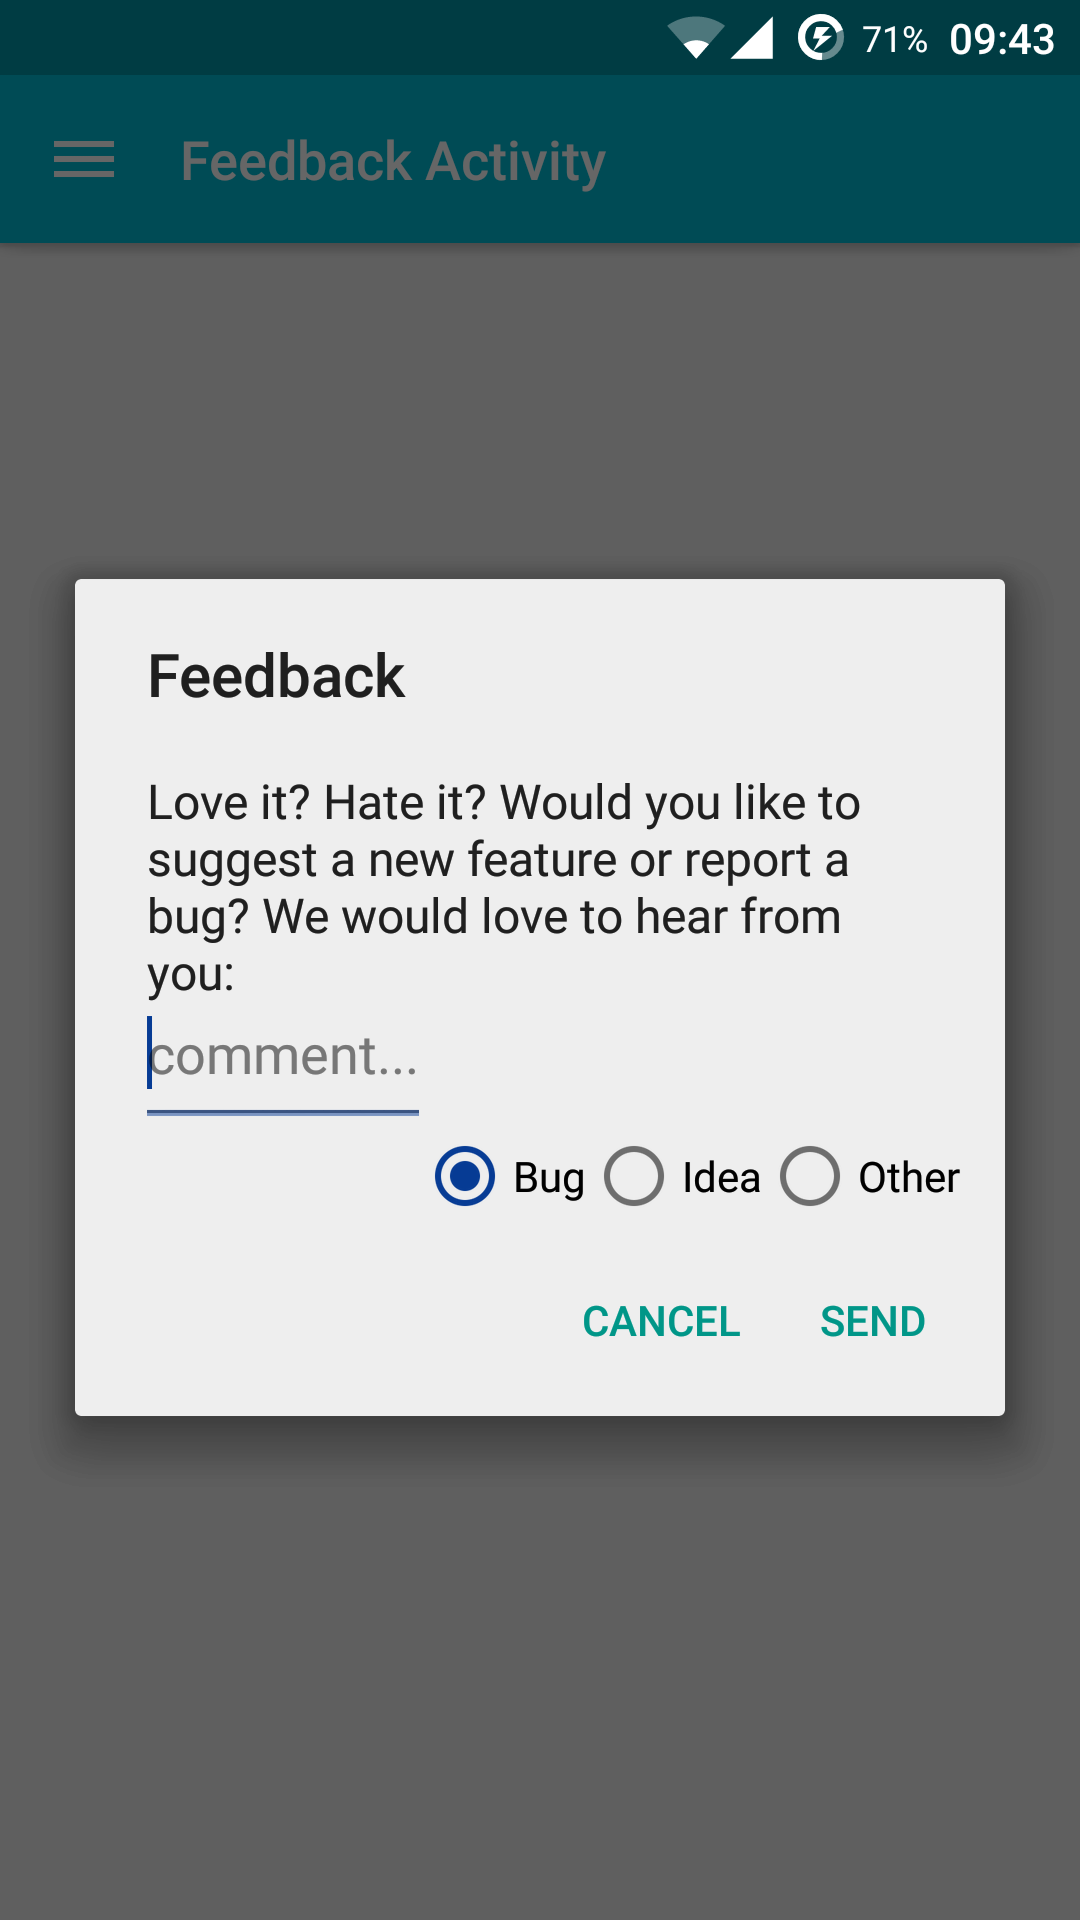
\includegraphics[width=\textwidth]{shot_feedback}
\caption{Feedback}
\label{fig:shot_feedback}
\end{minipage}
\hspace{1.5cm}
\begin{minipage}[b]{0.25\linewidth}
\centering
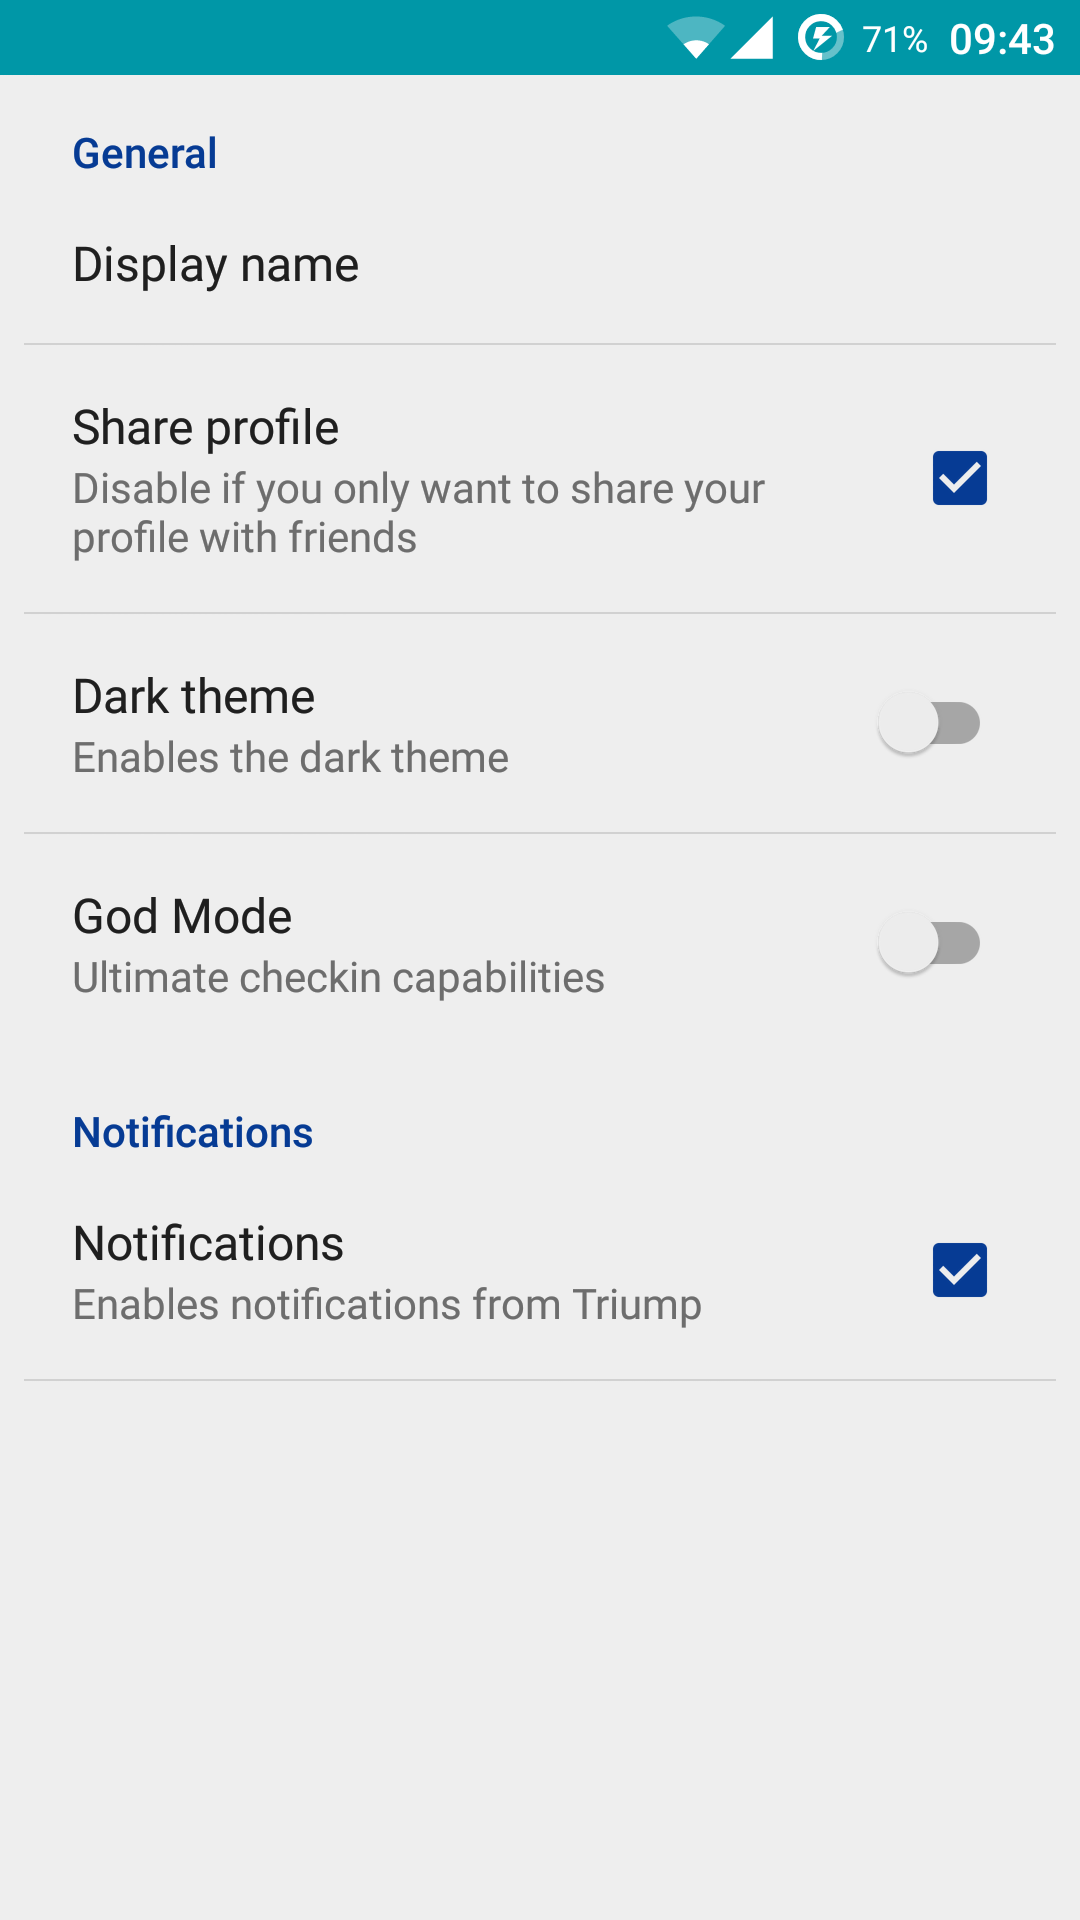
\includegraphics[width=\textwidth]{shot_instellingen}
\caption{Instellingen}
\label{fig:shot_instellingen}
\end{minipage}
\hspace{1.5cm}
\begin{minipage}[b]{0.25\linewidth}
\centering
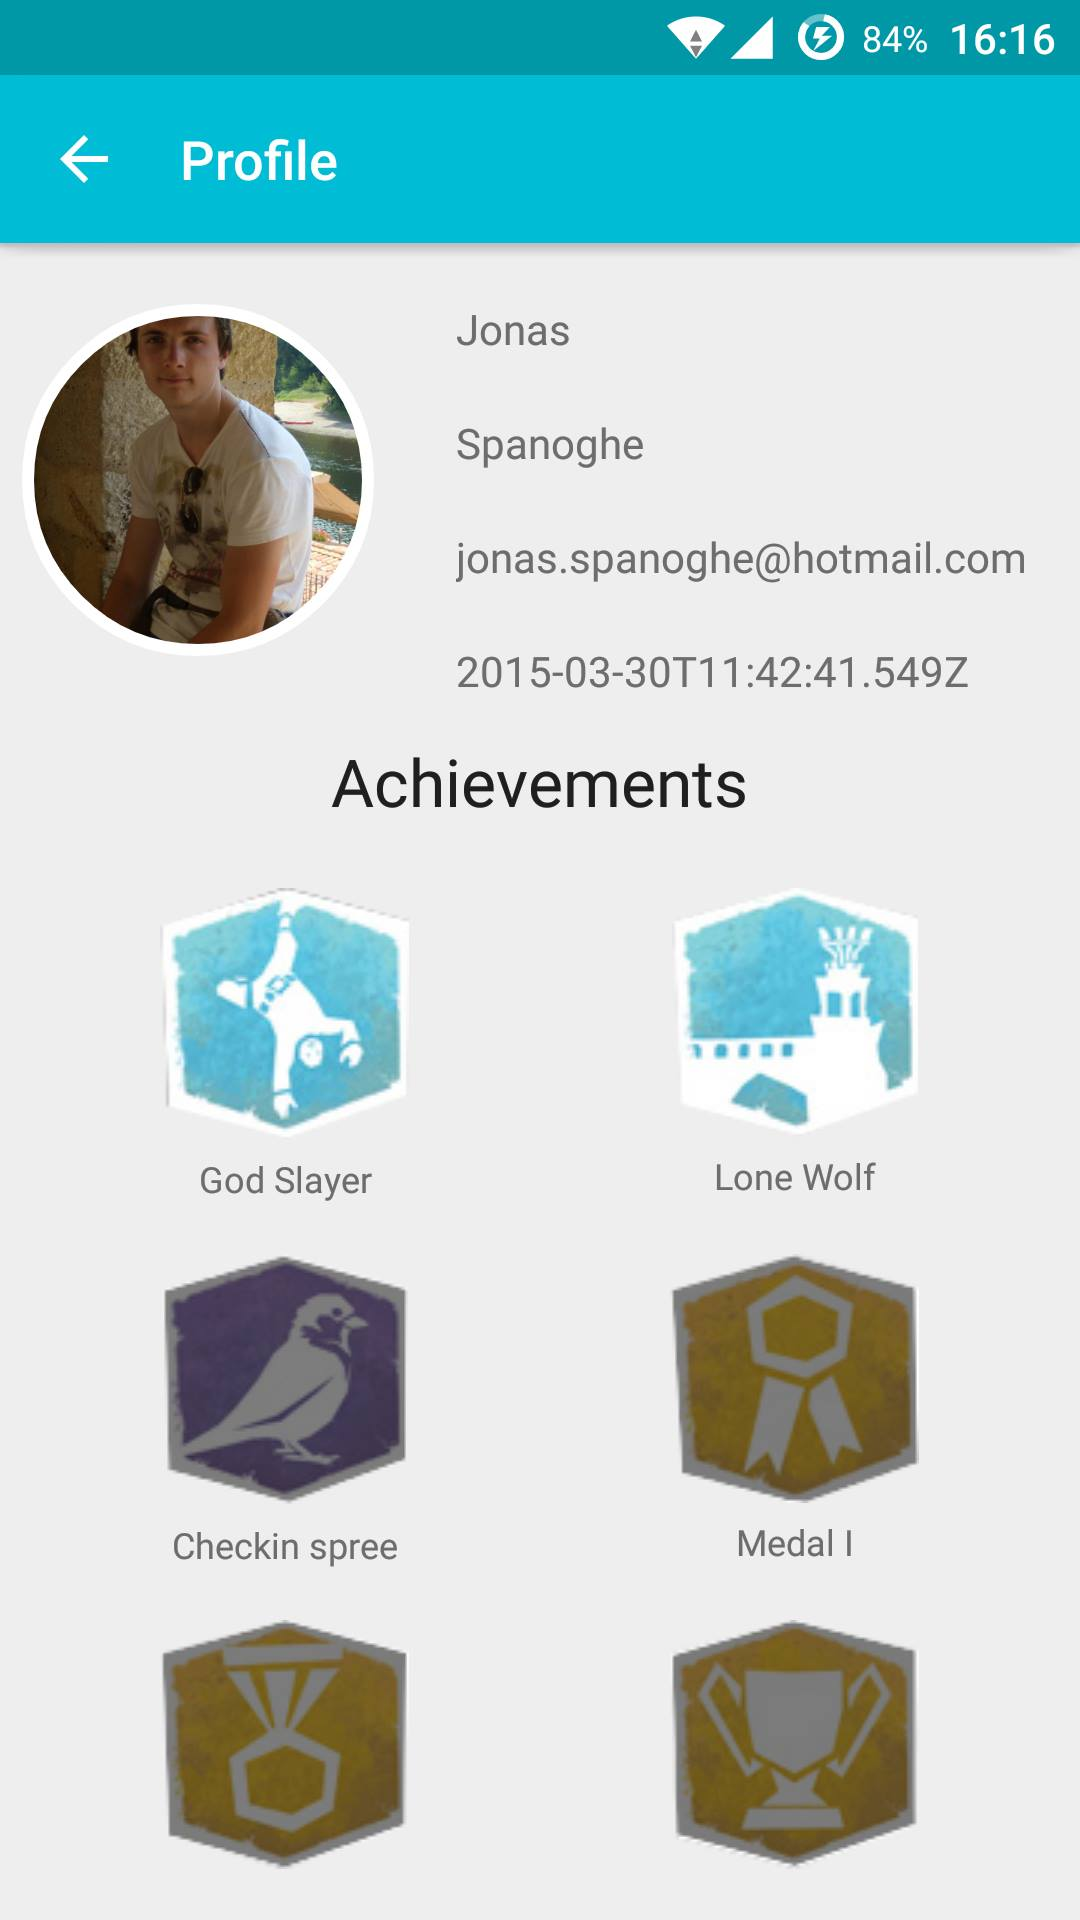
\includegraphics[width=\textwidth]{shot_profile}
\caption{Profiel}
\label{fig:shot_profile}
\end{minipage}
\end{figure}

\section{Webinterface}%Jonas -A
De website van Triump, die te bekijken is op triump.be, bestaat uit 2 delen. Enerzijds is er een deel waarvoor men niet dient ingelogd te zijn. Hier kan men informatie vinden over Triump, de applicatie downloaden en de ontwikkelaars contacteren . Anderzijds is er de interface voor gebruikers van Triump, waarvoor men ingelogd dient te zijn. Hier kan men groepen en evenementen bekijken, maar de belangrijkste functionaliteit van dit gedeelte is het registreren van een locatie.
Het registreren van een locatie is noodzakelijk indien men een officieel evenement wil organiseren.
\subsubsection{Publieke pagina's}
De publieke pagina's van de website zijn voornamelijk bedoeld ter promotie van Triump. Vanuit de startpagina kan genavigeerd worden naar `Contact' en `About' om meer informatie over Triump te verkrijgen. Via de sectie `Download' kan de applicatie gedownload worden. Dit is voornamelijk bedoeld voor de testgebruikers, vermits lancering op de Google App Store pas na uitvoerig testen mogelijk is. Testgebruikers kunnen de testversie downloaden via de website. Via `Sign up' kunnen gebruikers zich registreren om gebruik te kunnen maken van de webinterface voor Triump.\\
Op de Contact-pagina is er de mogelijkheid om feedback te geven en een mail te sturen.
Op de About-pagina vindt men algemene informatie over de applicatie.
\subsubsection{Inloggen}
Om de webinterface van Triump te kunnen gebruiken, dient men zich eerst te registreren. Hierna logt men dan in met de nieuwe account die men kan koppelen aan Foursquare.
\subsubsection{Registreren van locatie}
Nadat men is ingelogd kan men een locatie uit de Foursquare-database bij Triump registreren.
Momenteel is het enkel mogelijk om te zoeken naar locaties rondom Gent, aangezien de eerste testen van Triump daar gebeuren.
Om er zeker van te zijn dat het wel degelijk om de juiste locatie gaat, is er een link aanwezig die leidt naar de Fourquare-pagina van die locatie.
Vervolgens bevestigt de gebruiker de registratie en wordt een mail te gestuurd naar Triump met de details van de locatie. De registratie wordt geverifieerd en uiteindelijk goedgekeurd.
De gebruiker kan vervolgens een officiëel evenement organiseren voor deze locatie via de webinterface.
%\begin{figure}[H]
%	\centering
%	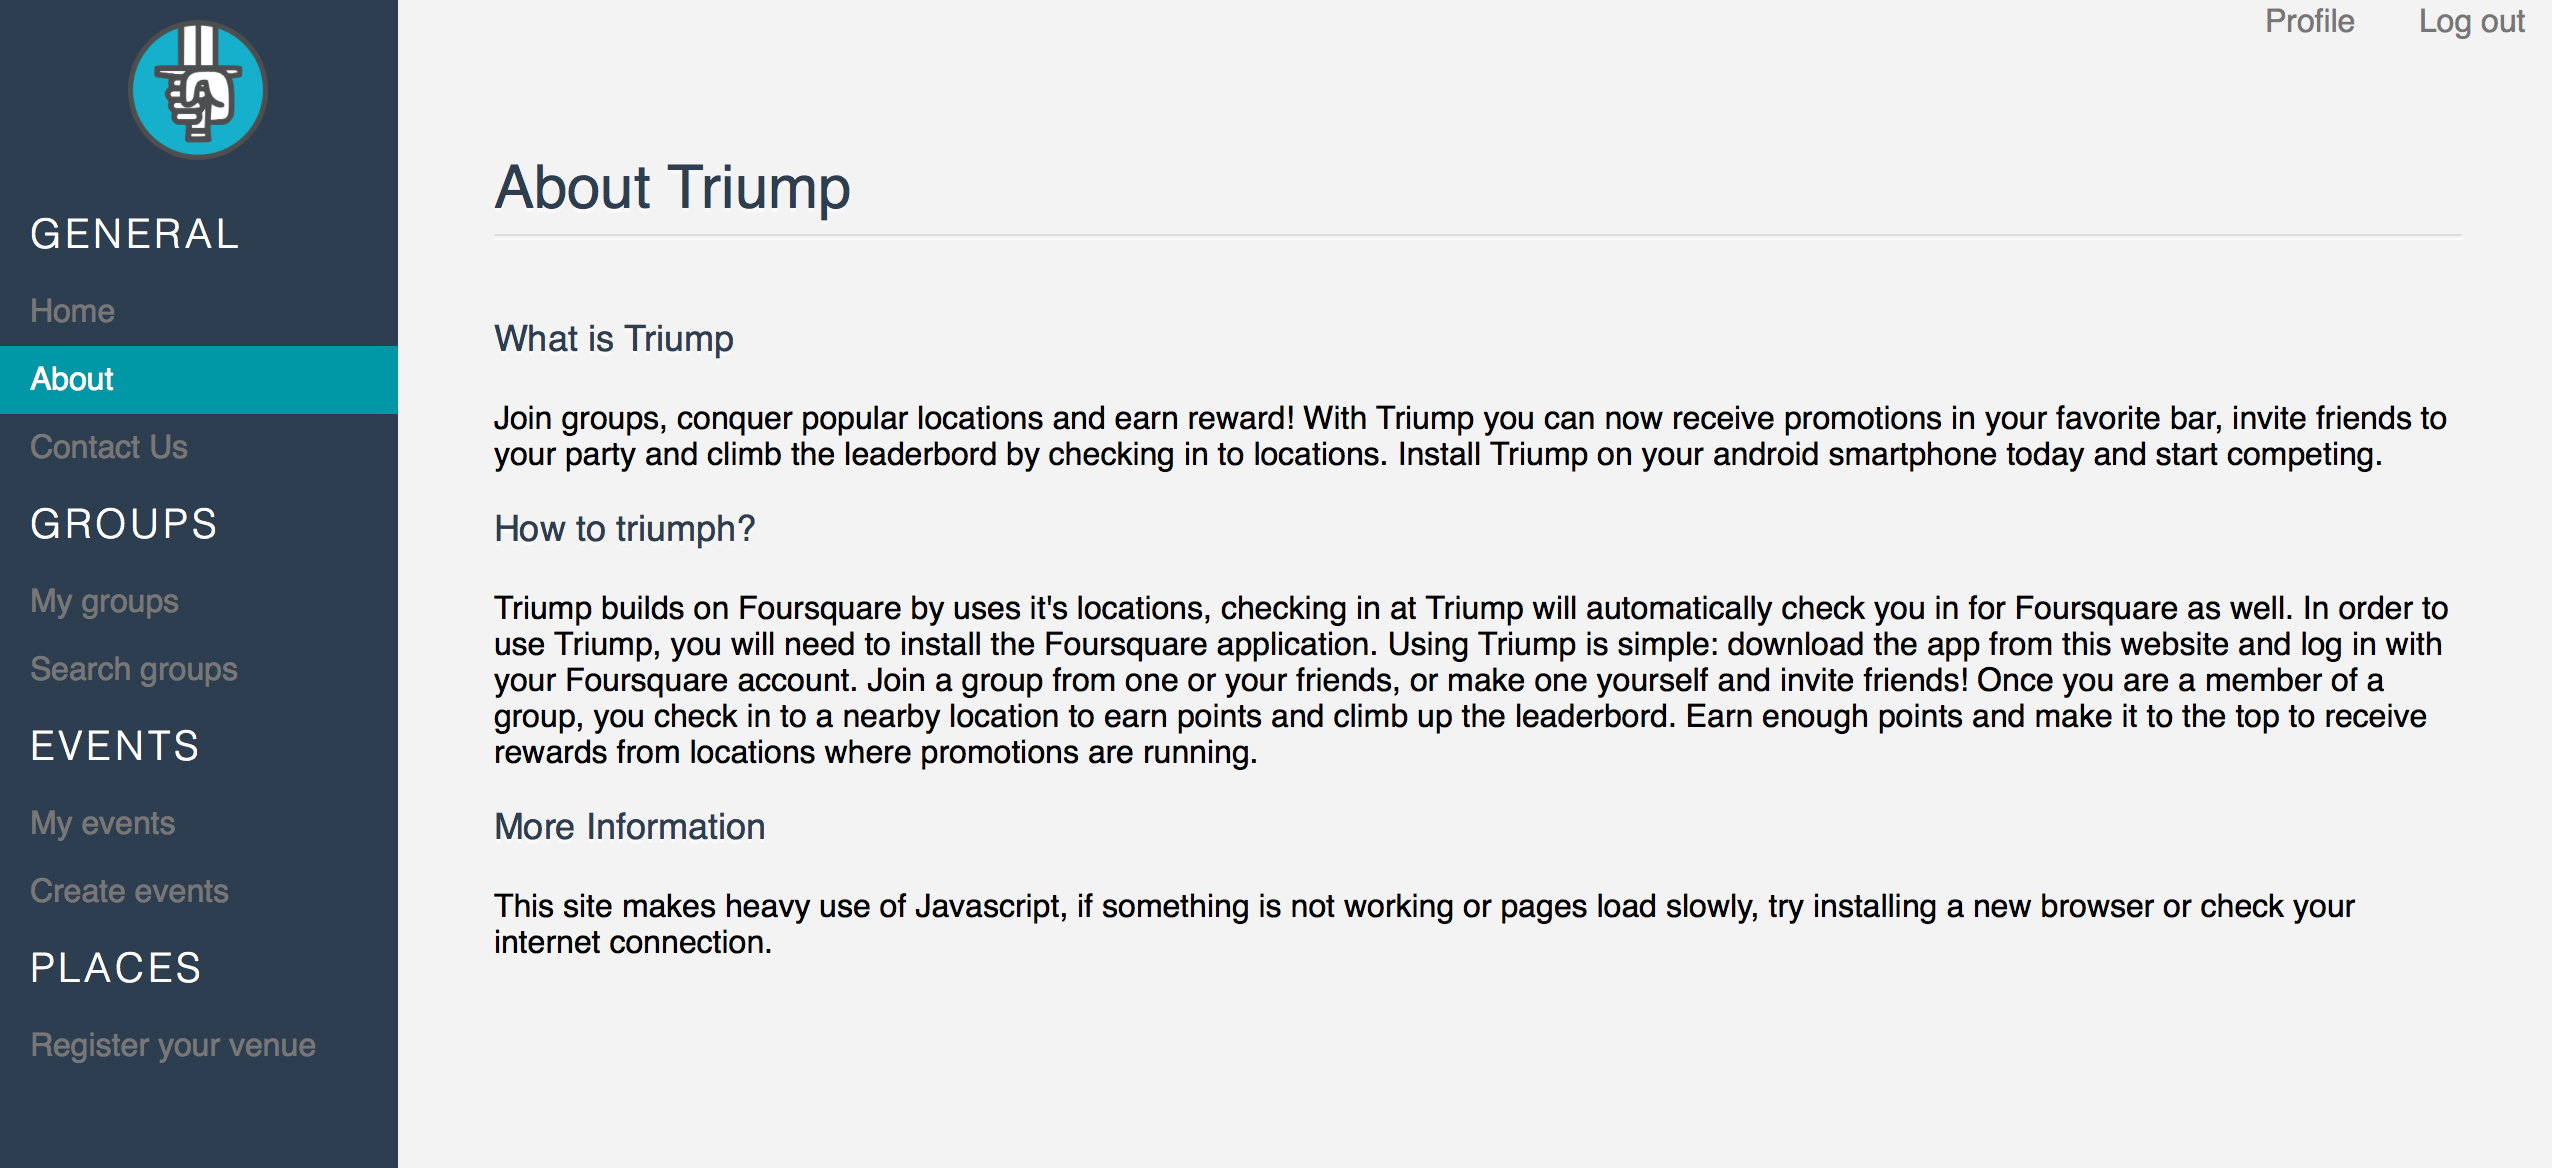
\includegraphics[scale=0.3]{about}
%	\caption{Publieke website }
%	\label{fig:about}
%\end{figure}

%\begin{figure}[H]
%	\centering
%	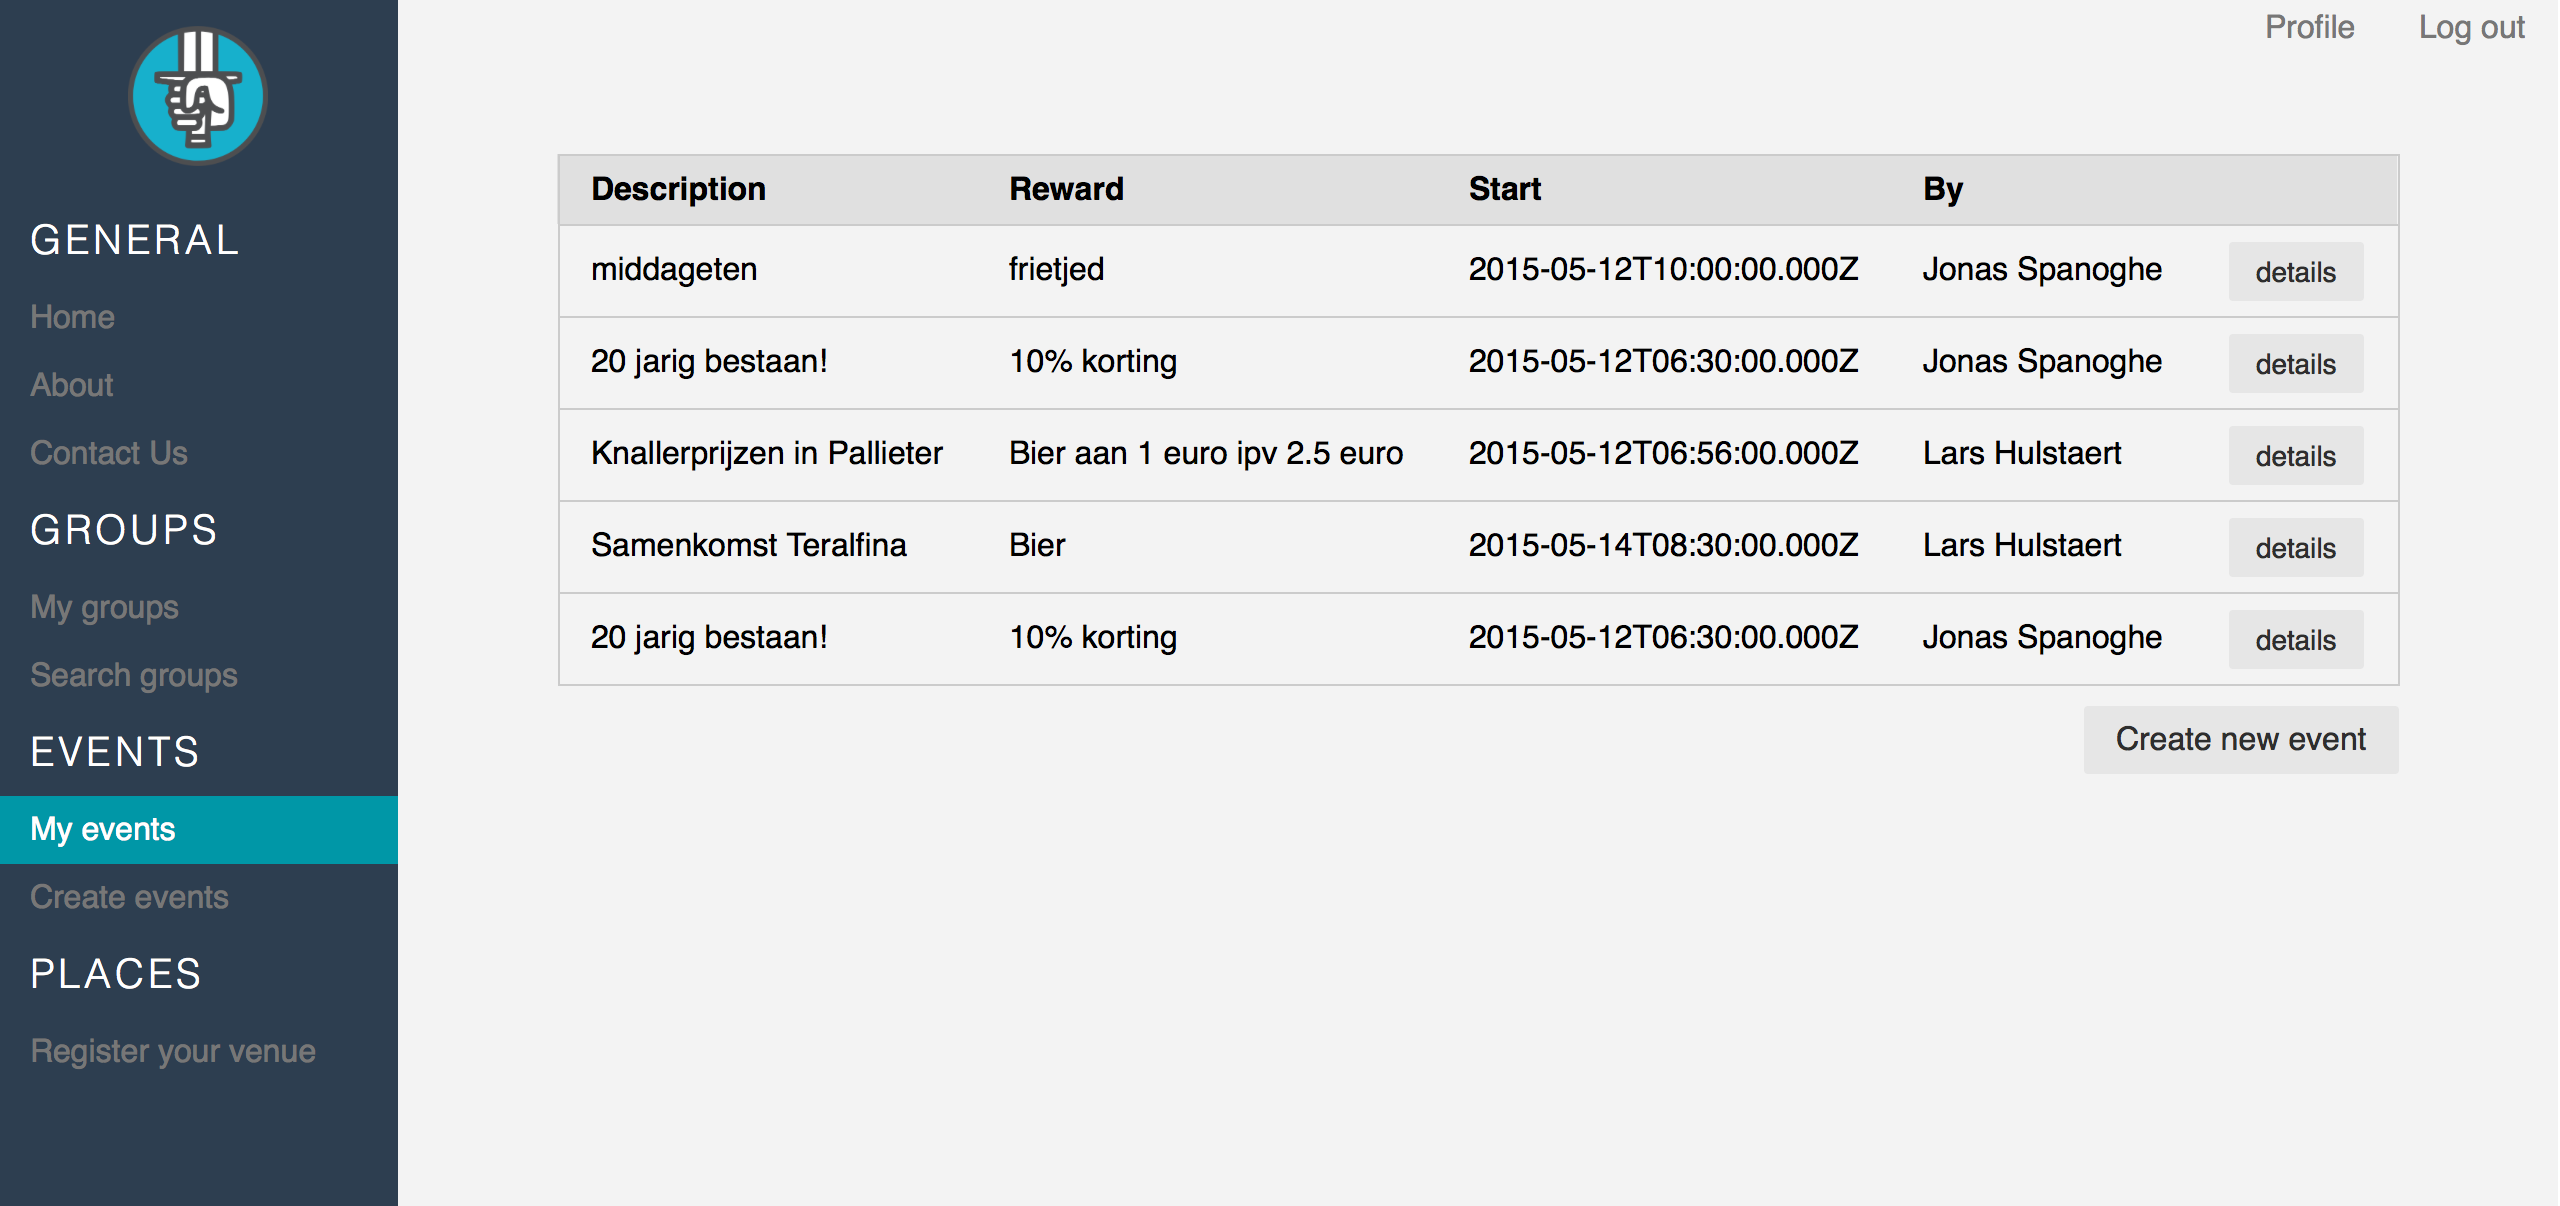
\includegraphics[scale=0.3]{events}
%	\caption{Webinterface }
%	\label{fig:events}
%\end{figure}

% Verschillende schermen tonen van webinterface en functionaliteit